\section{超伝導回路素子}
    サンプル作成に使用した超伝導回路素子の説明を包括的に行う。まずは超伝導共振器の導入を行う。
    \subsection{超伝導共振器}
    超伝導共振素子は量子コンピュータ\cite*{Goppl2008}や量子増幅器、光子メモリ\cite*{Pierre2014}、そして結合素子\cite*{Baust2015,Reuther2009}等様々なデバイスに応用されている。
        この章では超伝導体を用いた共振素子についてマイクロ波エンジニアリングに基づいて記述する。\cite*{Microwave}
        最も簡便な共振モデルは図のようなLC共振回路である。
        \begin{figure}[H]
            \centering
            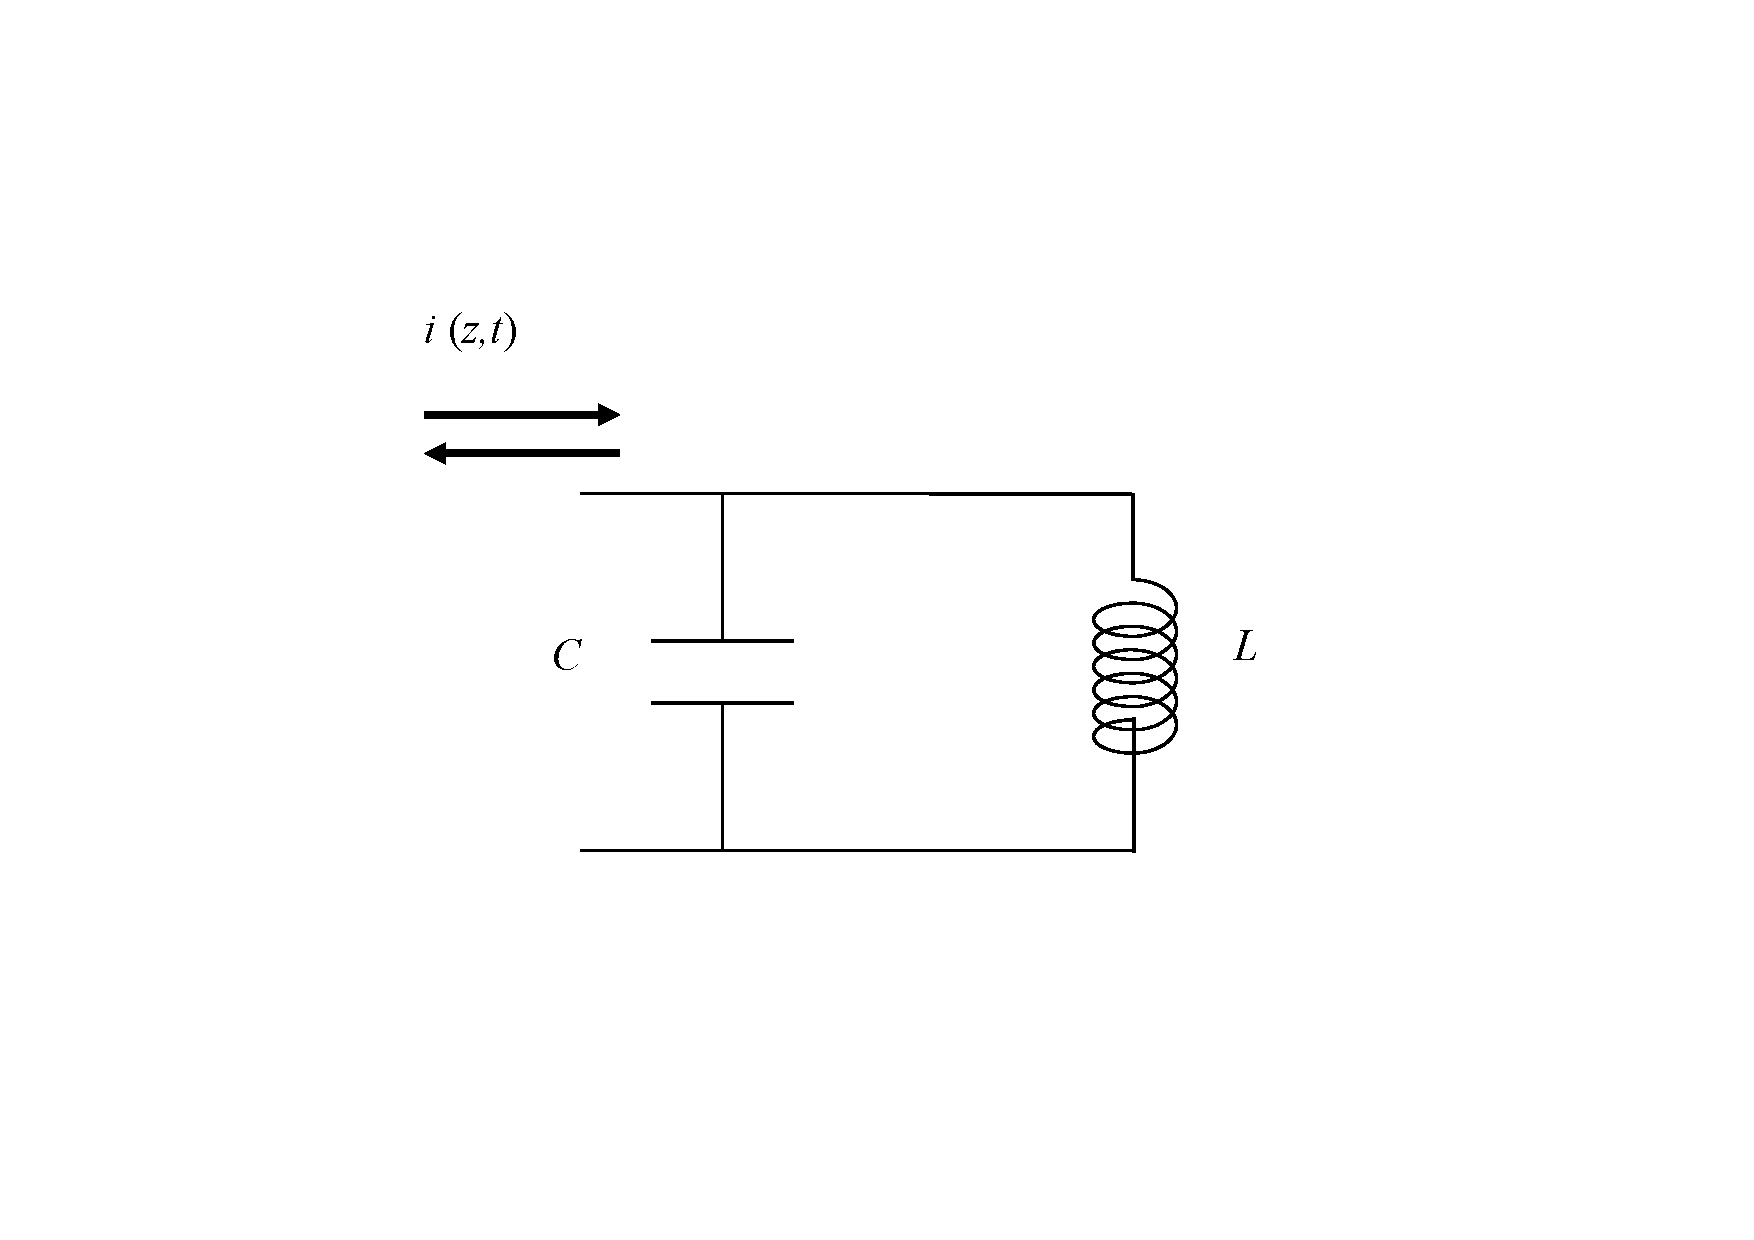
\includegraphics[width=9cm]{le.pdf}
            \caption{エネルギースペクトル}
        \end{figure}
        このとき共振周波数は回路のインダクタンスとキャパシタンスを用いて$\omega_0=1/\sqrt{LC}$と表現できる。
        図のような平行共振回路の複素インピーダンスは
        \begin{equation}
            Z_{i n}=\frac{1}{\frac{1}{R}+\frac{1}{j \omega L}+j \omega C}
        \end{equation}
        のように記述できる。この時共振回路のパワーはオームの法則により
        \begin{equation}
            P_{i n}=\frac{1}{2} V I^{*}=\frac{1}{2}|V|^{2}\left(\frac{1}{R}+\frac{j}{\omega L}-j \omega C\right)
            \end{equation}
        と表現することができる。LC共振回路において抵抗は損失である。損失分のパワーは
        \begin{equation}
            P_{\text {loss }}=\frac{1}{2} \frac{|V|^{2}}{R}
        \end{equation}
        と表現される。また、共振回路中キャパシタンス及びインダクタンスに蓄えられる平均エネルギーはそれぞれ
        \begin{equation}
            \begin{array}{l}
            W_{m}=\frac{1}{4}|V|^{2} \frac{1}{\omega^{2} L} \\
            W_{e}=\frac{1}{4}|V|^{2} \frac{1}{\omega^{2} L} .
            \end{array}
            \end{equation}
        と記述することができる。共振器の性能を表す特徴量であるQ値は損失に対して蓄えられるエネルギー量の指標であり、次のように表現される。
        \begin{equation}
            Q_{\text {int }}=\omega \frac{共振回路の平均エネルギー}{単位時間あたりの損失エネルギー}
        \end{equation}
        上記の式を代入することで
        \begin{equation}
            Q_{\text {int }}=\omega \frac{W_{e}+W_{m}}{P_{\text {loss }}}=\omega_{0} \frac{2 W_{m}}{P_{\text {loss }}}=\frac{R}{\omega_{0} L}=\omega_{0} R C .
        \end{equation}
        のように記述できる。ここでQ値にintと添え字をつけたがこれは共振回路自身のQ値を表している。しかしながら回路としては共振回路に接続されることで生じるQ値も存在している。これを$Q_{ext}$と表現すると、回路全体のQ値は
        \begin{equation}
            \frac{1}{Q_{\text {total }}}=\frac{1}{Q_{\text {int }}}+\frac{1}{Q_{\text {ext }}}
        \end{equation}
        と表現される。

        ここで共振回路の観測可能量について説明をする。当研究室では共振器の測定にVNA(ベクトルネットワークアナライザ)を用いている。この測定機器はローカルオシレーターを内蔵しており、入力信号と反射信号そして透過信号を参照することにより被測定物の散乱パラメータを測定することができる。
        散乱パラメータは共振回路の共振周波数及びQ値を用いることにより、次のように表現できる。
        \begin{equation}
            S_{21}(f)=\frac{Q_{total} / Q_{ext}}{1+2 j Q_{total}\left(f-f_{0}\right) / f_{0}}
        \end{equation}
        また透過係数は
        \begin{equation}
            S_{11}(f)=1-\frac{Q_{m} / Q_{c}}{1+2 j Q_{m}\left(f-f_{0}\right) / f_{0}}
        \end{equation}
        である。測定では透過係数及び反射係数の絶対値を上記関数でフィットし、共振回路を評価する。

        次に超伝導共振器として特に利用される回路デザインとして超伝導分布定数回路及び超伝導準集中定数共振回路について記述する。
        \subsubsection{超伝導分布定数回路}
            最も使用頻度の高いデザインは平面型共振回路(CPW)である。
            \begin{figure}[H]
                \centering
                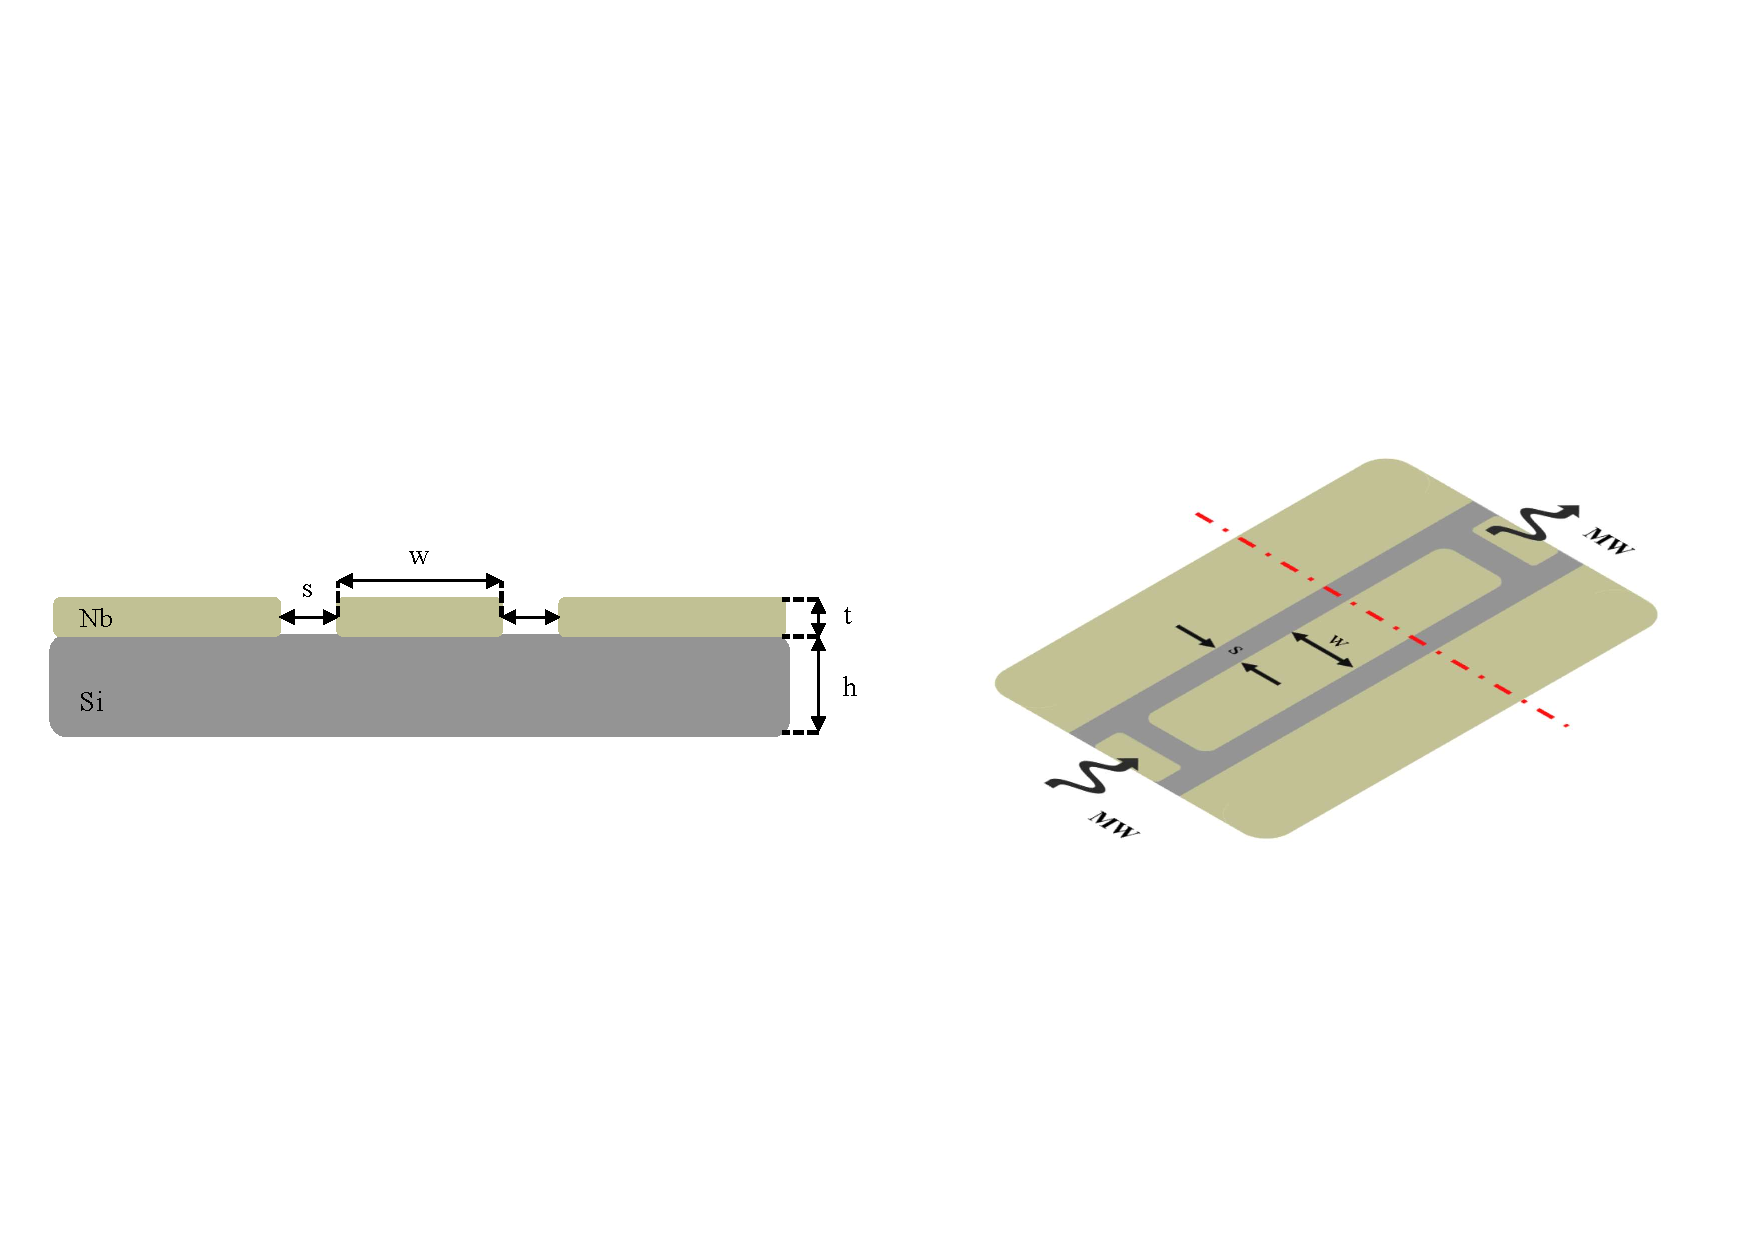
\includegraphics[width=14cm]{cpw2.pdf}
                \caption{CPW型断面図}
            \end{figure}
            CPW型共振回路の外観及び断面図を示した。CPW型回路は図中に示されたパラメータを調節することで回路のインピーダンスを適切に設計することができる。比較的簡便に高いQ値を持った共振回路を作成することができるため、超伝導量子エレクトロニクスの分野では頻繁に利用されている。当研究室ではSiの誘電率$\epsilon_r=11.9$を設計パラメータとして$s=6,w=10,t=50nm,h=450nm$を使用している。
            \begin{figure}[H]
                \centering
                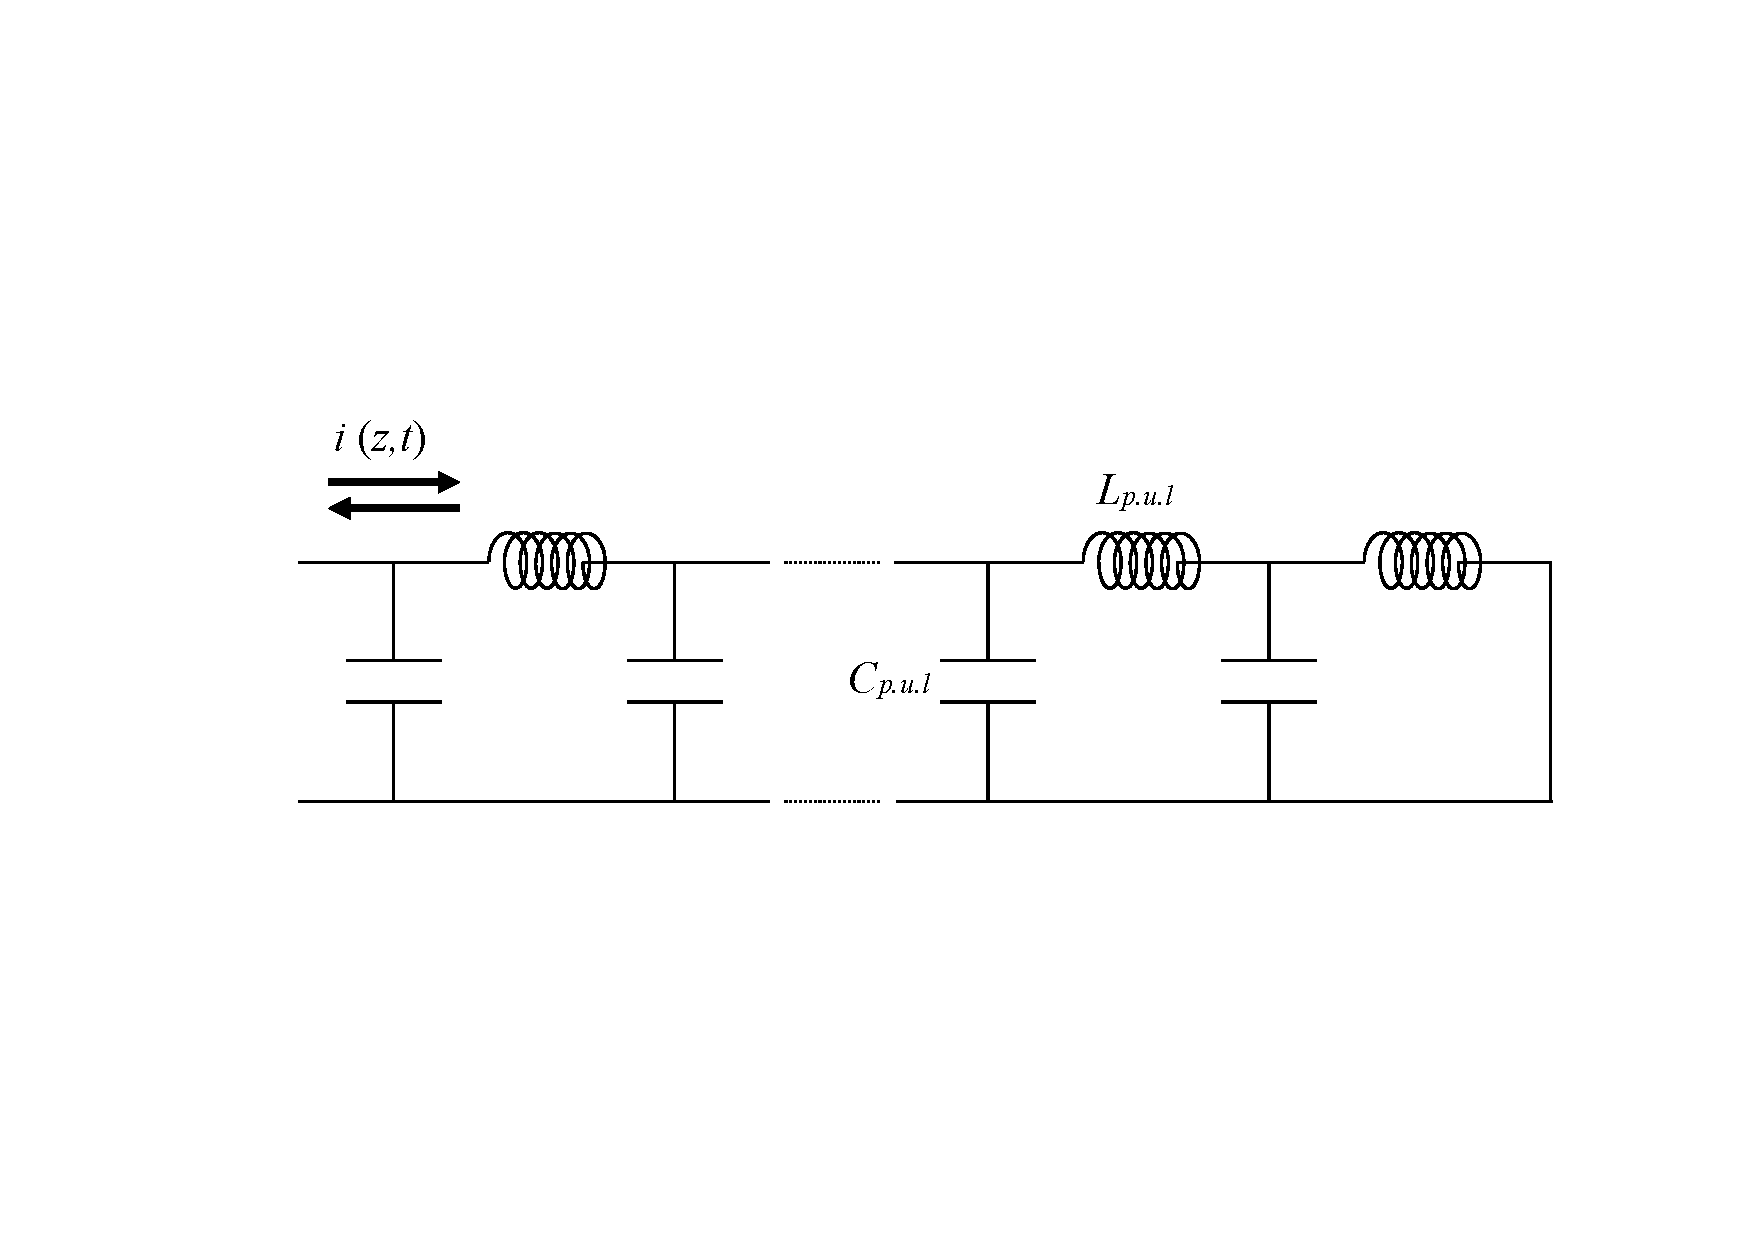
\includegraphics[width=9cm]{cpw.pdf}
                \caption{分布定数回路}
            \end{figure}
            分布定数回路は単位長さあたりのインピーダンスが一定に保たれているため、損失が少ない。単位長さあたりのキャパシタンスとインダクタンスをそれぞれ$C_l$、$L_l$とすると回路全体の共振周波数は
            \begin{equation}
                f_{0}=\frac{1}{2l\sqrt{L_l C_l}}
                \end{equation}
            と表記できる。ここで$2l=\lambda_0$である\cite*{Goppl2008,Besedin2018,inomata}。CPW型共振器において単位長さあたりのキャパシタンス及びインダクタンスはコンフォーマルマッピングという計算方法によって以下のように求めることが可能である。
            \begin{equation}
                L_{\ell}=\frac{\mu_{0}}{4} \frac{K\left(k_{0}^{\prime}\right)}{K\left(k_{0}\right)}
            \end{equation}
            \begin{equation}
                C_{\ell}=4 \epsilon_{0} \epsilon_{\mathrm{eff}} \frac{K\left(k_{0}\right)}{K\left(k_{0}^{\prime}\right)}
            \end{equation}
            \begin{equation}
                \begin{array}{l}
                k_{0}=\frac{w}{w+2 s} \\
                k_{0}^{\prime}=\sqrt{1-k_{0}^{2}}
                \end{array}
            \end{equation}
            ここでKは第一種楕円積分を表している。実際には超伝導体を用いているため、単位長さあたりのカイネティックインダクタンスも考慮しなければならない。サンプルの設計においては上記幾何学構造に依存するキャパシタンス及びインダクタンスを求めた後、カイネティックインダクタンスを別途求める必要があることに注意が必要である。すなわち
            \begin{equation}
                L(t, T)=L_{g}(t)+L_{k}(t, T)
            \end{equation}
            ここで前項が幾何学的構造に依存するインダクタンス、2項目がカイネティックインダクタンスである。カイネティックインダクタンスについてはさらに
            \begin{equation}
                L_{k}=\frac{\mu_{0}}{\pi^{2}}(\lambda / w) \ln (4 w / t) \frac{\sinh (t / \lambda)}{\cosh (t / \lambda)-1}
            \end{equation}
            と表現することができる。ここで$\mu_0$は真空の透磁率であり、$\lambda_0$は超伝導体薄膜に置ける磁場侵入長である。磁場侵入長$\lambda_0$は超伝導体の転移温度に於ける超伝導エネルギーギャップに依存するため、物質固有の値である。続いて超伝導準集中定数共振回路について解説する。
        \subsubsection{超伝導準集中定数回路}
            超伝導準集中定数回路は局所的に大きなキャパシタンスとインダクタンスを設けることでLC共振を実現している。回路デザインは下記のようにミアンダインダクタンスとインターデジタルキャパシタと呼ばれる幾何学的構造を作ることでキャパシタンスとインダクタンスを別々に作り出すという方法が一般的である。
        \begin{figure}[H]
            \centering
            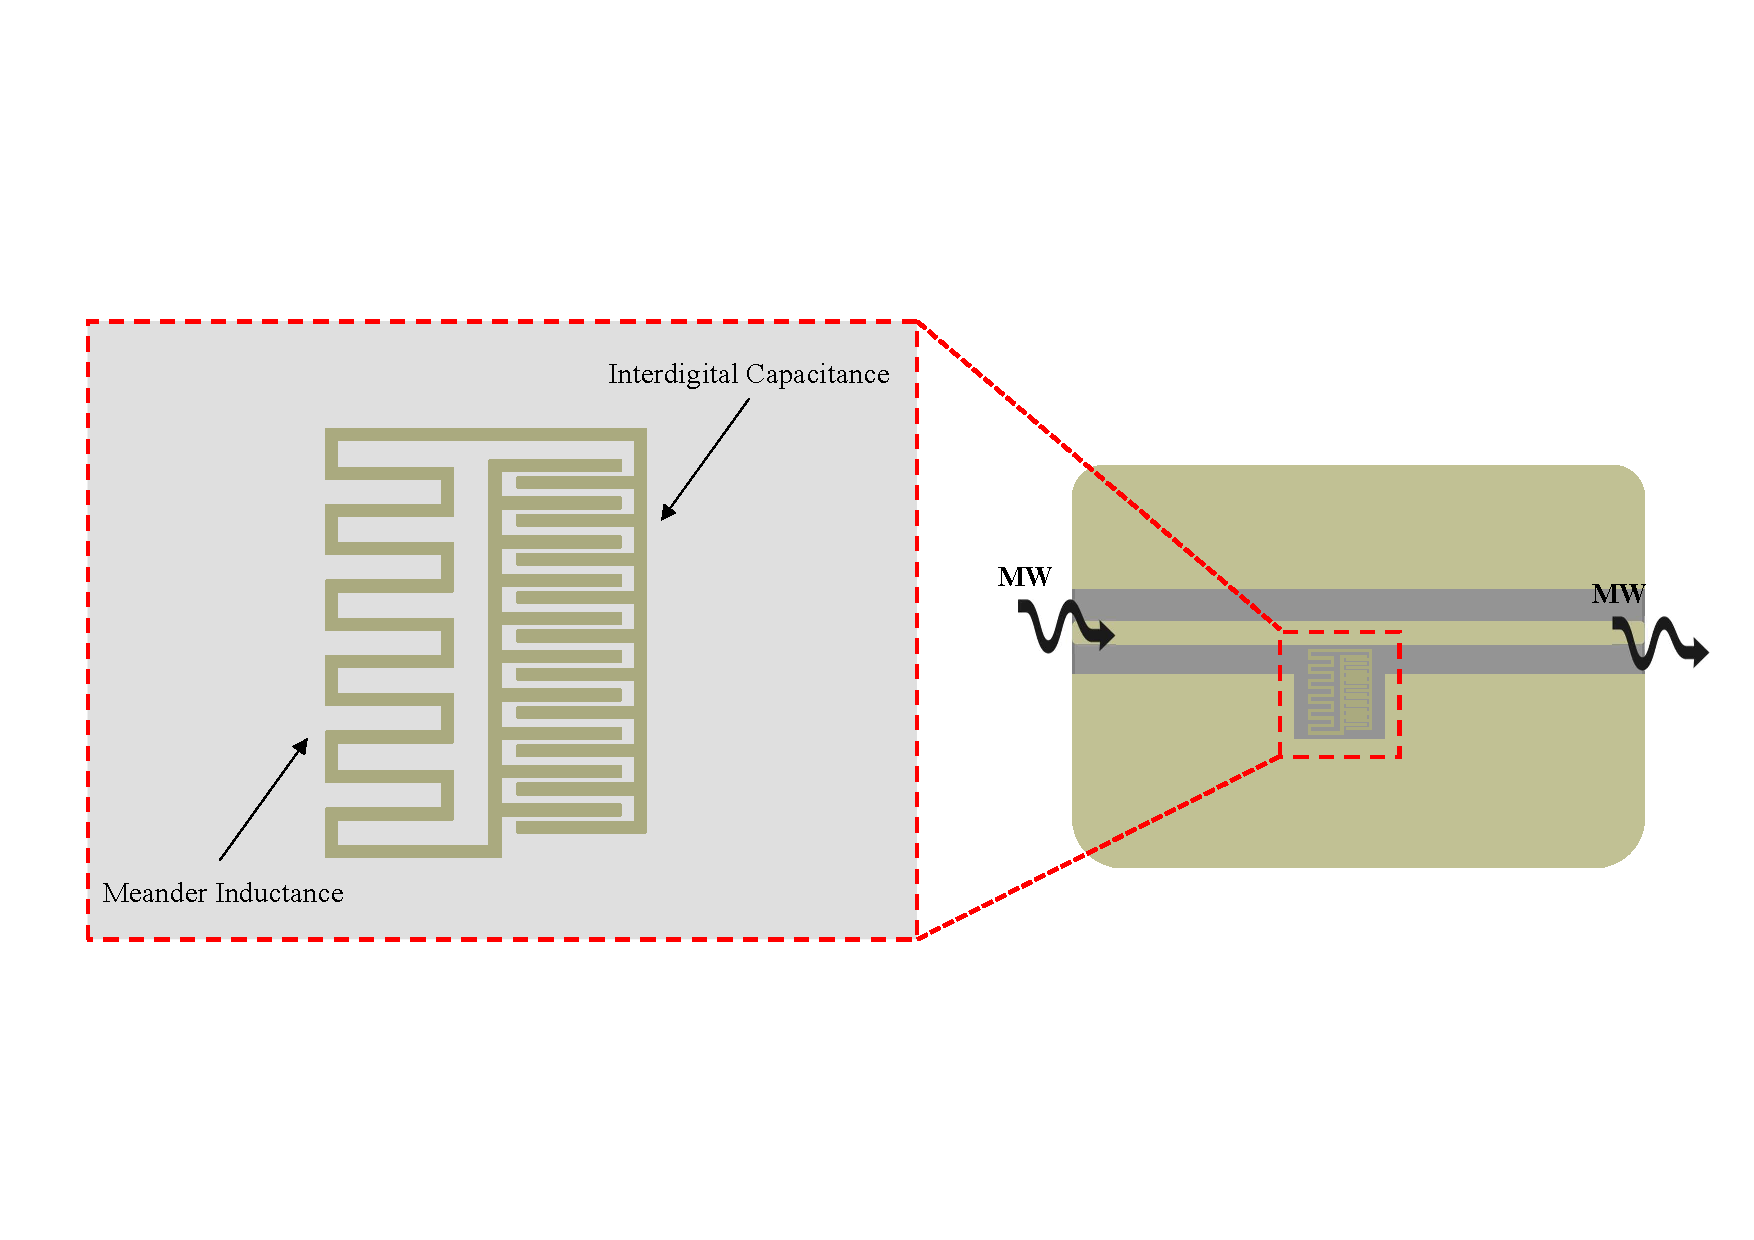
\includegraphics[width=14cm]{lumpedelement.pdf}
            \caption{超伝導準集中定数回路}
        \end{figure}
            \begin{figure}[H]
                \centering
                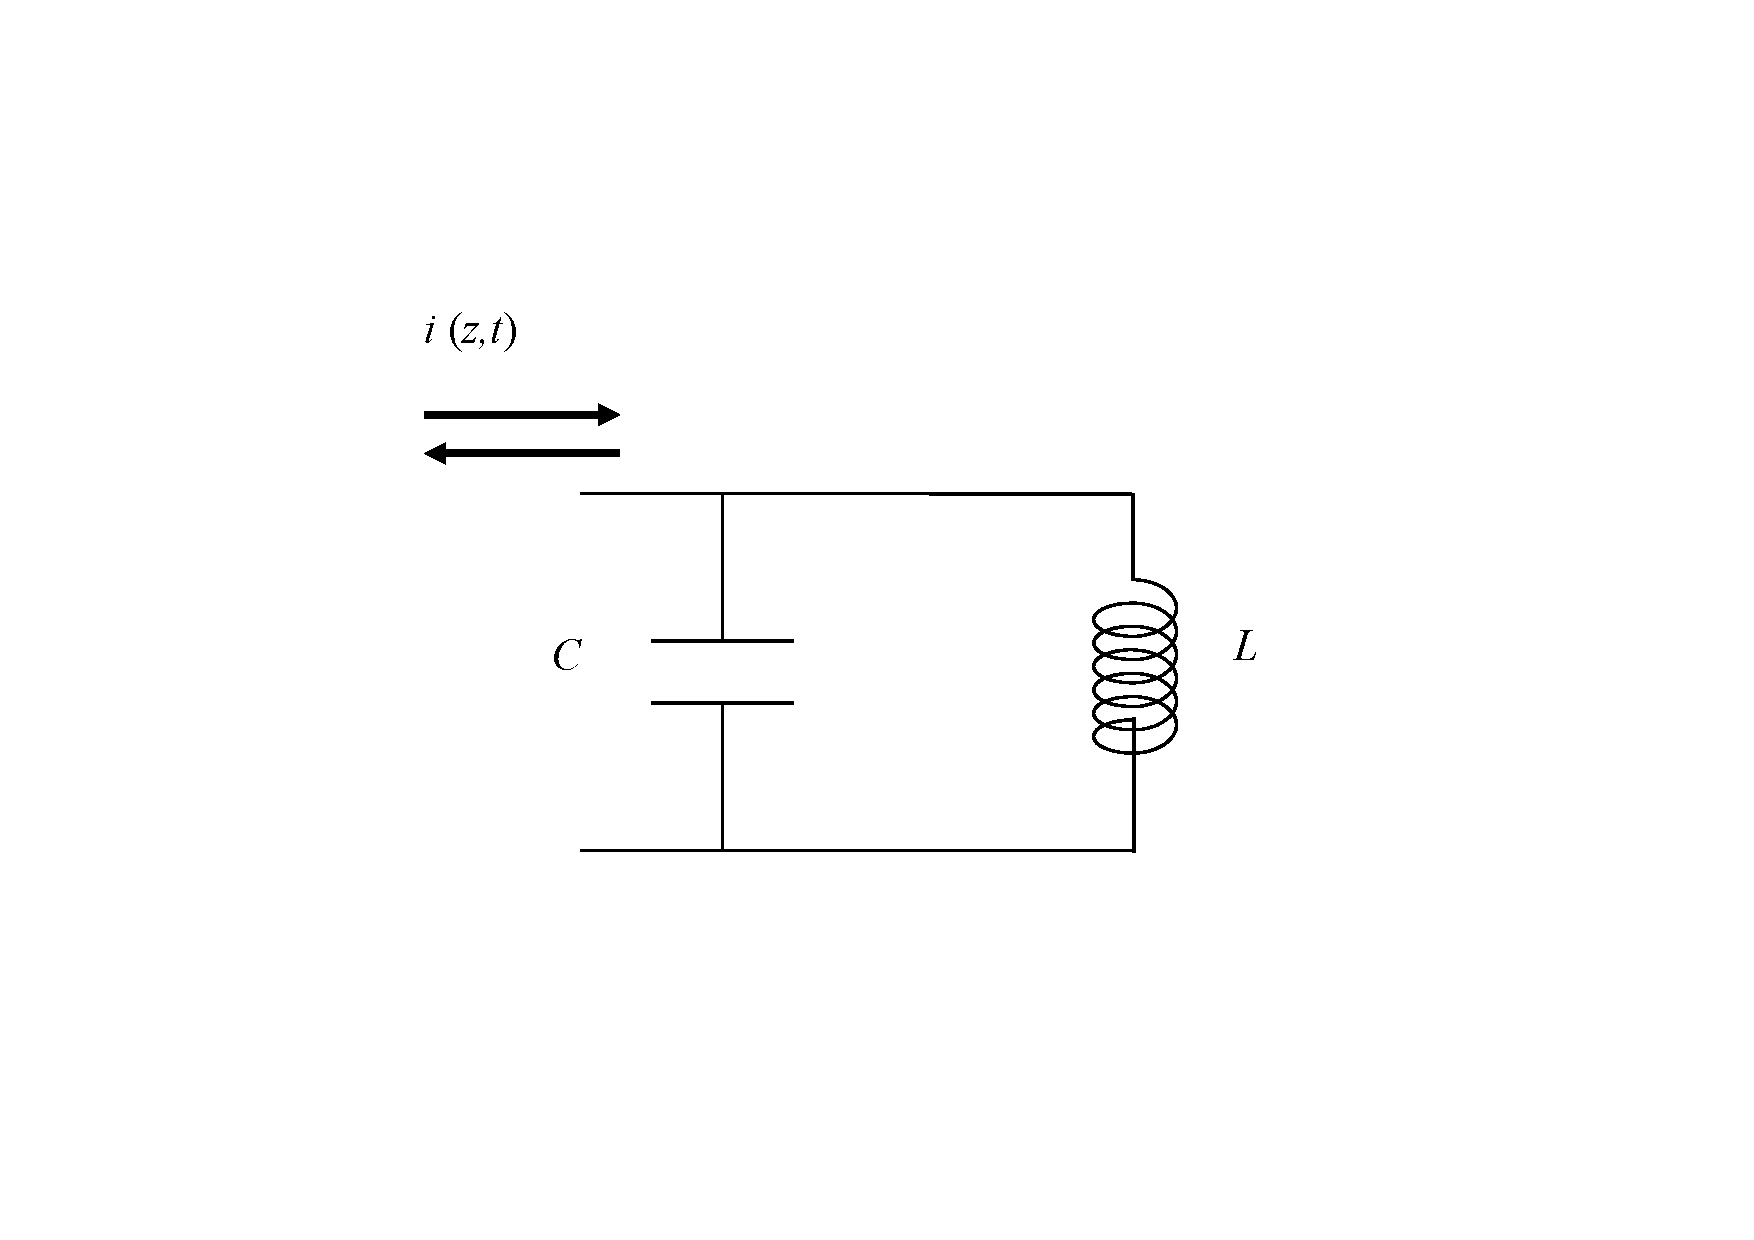
\includegraphics[width=9cm]{le.pdf}
                \caption{エネルギースペクトル}
            \end{figure}
            インターデジタルキャパシタンス及びミアンダインダクタンスの詳細な計算方法については付録に記載する。
    \subsection{ジョセフソン接合}
            ここまで超伝導共振器について解説してきた。ここでは超電導量子エレクトロニクスにおいて最も重要な素子、ジョセフソン接合について記述する。
            ジョセフソン接合は量子ビットやJPA(ジョセフソンパラメトリック増幅器)や結合素子等、超伝導共振素子と同じく幅広く利用されている素子である。
            量子ビットを作る際においてはジョセフソン接合がもたらす非調和性により、擬似的に2準位原子を作り出すことを可能にしている。本稿の的テーマである結合素子においてもジョセフソン接合が非常に重要な素子となる。本稿においてはrf-SQUID及びdc-SQUIDを構成する素子としてジョセフソン接合を導入するが、それぞれの素子の説明を行う前にジョセフソン接合の基本的な原理をこの章で説明する。
            \begin{figure}[H]
                \centering
                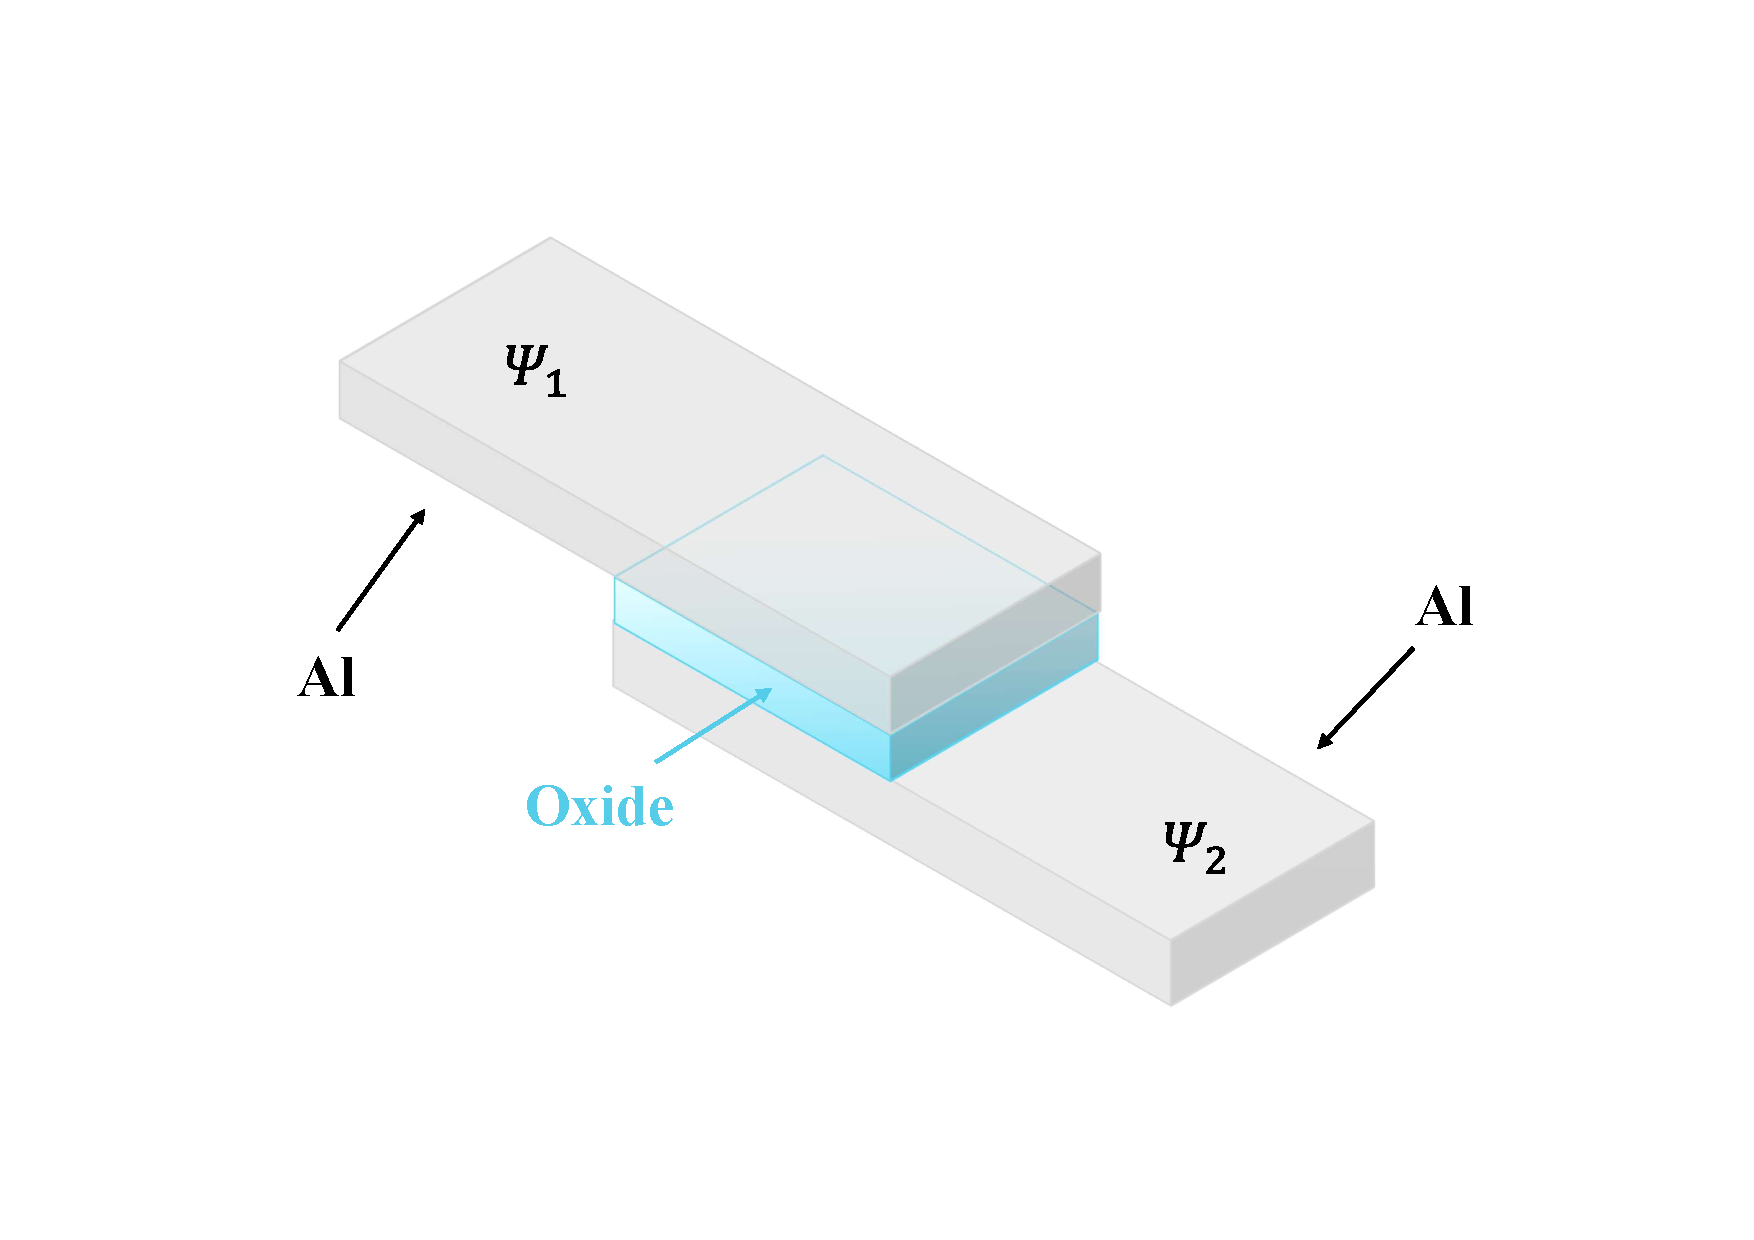
\includegraphics[width=9cm]{jj.pdf}
                \caption{ジョセフソン接合}
            \end{figure}
            ジョセフソン接合の形成方法はいくつかあるが、当研究室で採用している方法はSIS(超伝導体-絶縁体-超伝導体)型である。
            超伝導体間にアルミナ(Al2O3)を挟むことでジョセフソン接合を形成している
            ここではjosephson接合による物理的効果を理論から解説していくこととする。

            \begin{figure}[H]
                \begin{minipage}[t]{0.5\columnwidth}
                    \centering
                    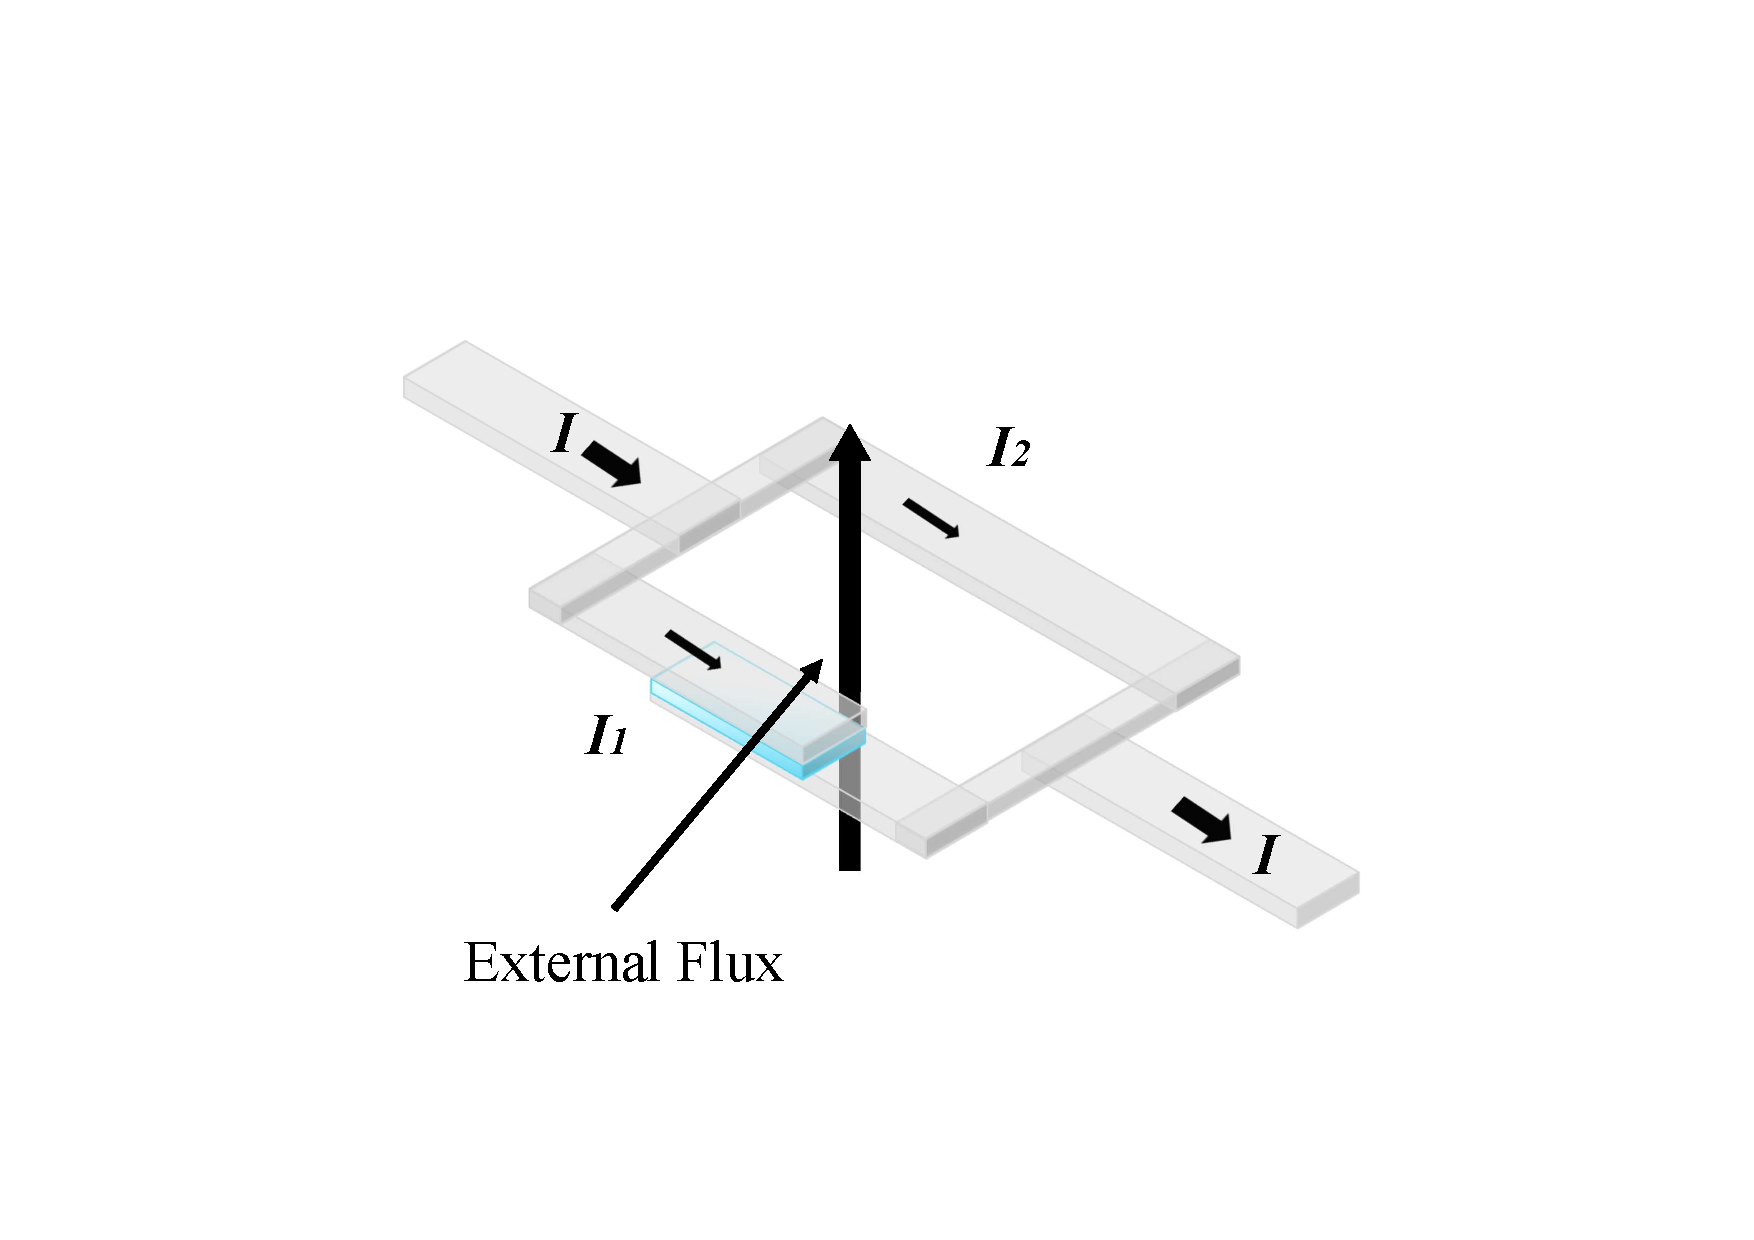
\includegraphics[clip, width=1.0\columnwidth]{rfsquid.pdf}
                    \caption{rf-SQUID}
                \end{minipage}%
                \begin{minipage}[t]{0.5\columnwidth}
                    \centering
                    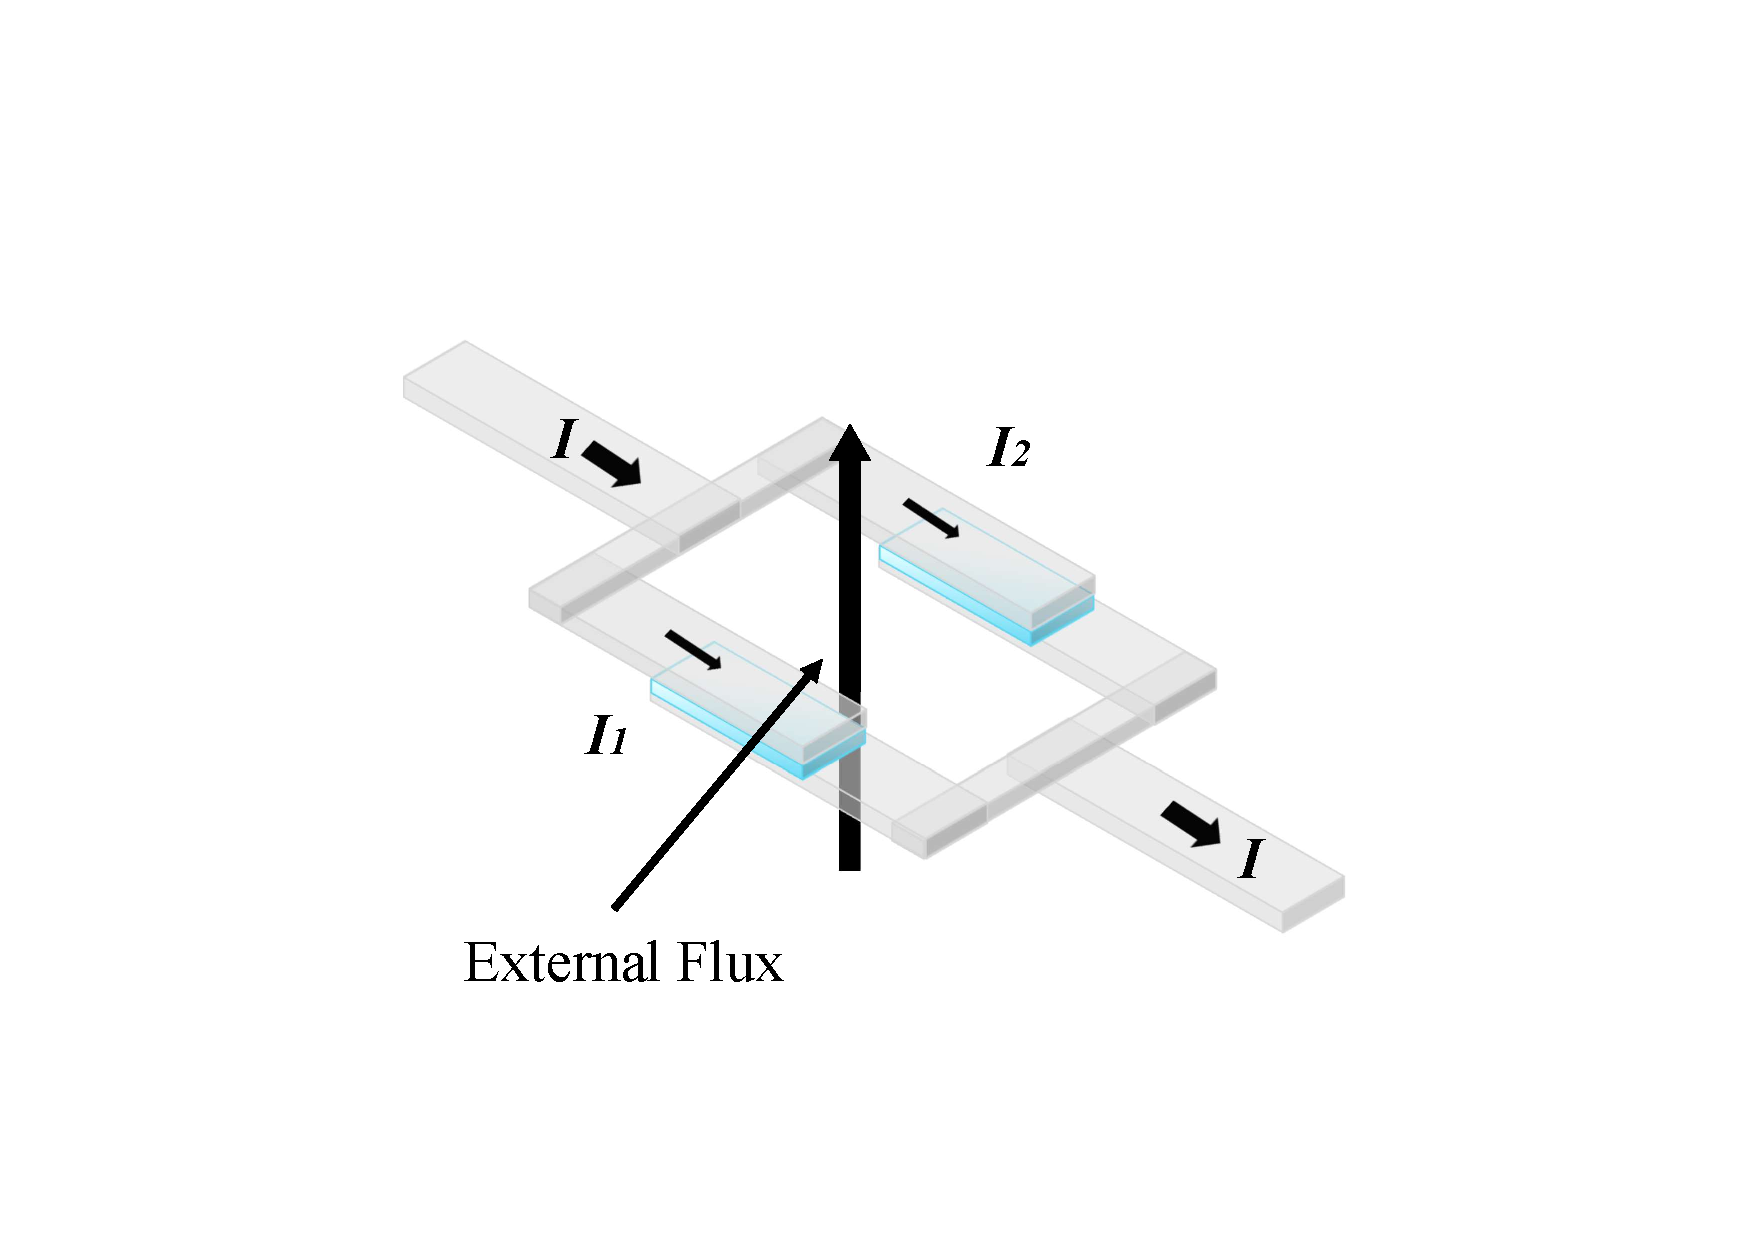
\includegraphics[clip, width=1.0\columnwidth]{dcsquid.pdf}
                    \caption{dc-SQUID}
                \end{minipage}
            \end{figure}
            超伝導状態になった金属中の粒子は
            この接合により生じsる物理的現象を、発見者の名に因んでjosephson効果と呼ぶ。
            この現象は大別するとACjosephson効果、DCjosephson効果の2つに分けることができる。
            この2つの効果についてGL理論から解説を始めることとする。
            \subsubsection{dc josephson効果}
                josephsonが1962年に行った理論的予言によれば、2つの超伝導体の間にゼロ電圧下で以下のような超伝導電流が流れるとしている。
                \begin{equation*}
                    I_s = I_c \sin(\Delta \psi)
                \end{equation*}
                ここで$\Delta \psi$とはGL波動関数のs位相差である。:また、臨界電流$I_c$は接合に流すことのできる、最大の超伝導電流である。
                彼はさらに接合に電位差vが生じているときに位相差が次のように振動すると予言した。
                \begin{equation*}
                    \frac{d(\Delta \psi)}{dt} = \frac{2eV}{\hbar}
                \end{equation*}
                これにより、電流は振幅を臨界電流$I_c$、周波数を$\nu = \frac{2eV}{h}$の交流となる。
                つまり、この電流変化はエネルギー$h\nu$でクーパー対が接合を通過するエネルギーと一致していることがわかる。
                以上2つの関係式によりこの接合により蓄えられるエネルギーは
                \begin{eqnarray}
                    \int_0^{t} (I_s V)dt&=&\int_{0}^{\delta} I_s(\hbar/2e)d\delta\\
                    &=&E_j(1-\cos (\delta))\\
                \end{eqnarray}
                と表現することができる。ここで$E_j=\hbar I_c/2e$である。
    \subsection{rf-SQUID}
                rf-SQUIDは
    \subsection{dc-SQUID}
        dc-SQUIDは超伝導ループ両枝にジョセフソン接合を一つずつ導入したものである。磁束量子干渉計とも呼ばれ広範囲の分野で応用されている素子である。代表的な例を上げれば重力波の観測やなどに使われている。外部磁場に非常に敏感であり
        dc-SQUIDを導入する意図はrf-SQUIDのジョセフソン接合を可変にするためである。これによりrf-SQUIDのジョセフソンインダクタンスは外部磁場に対し変化する。
        \begin{figure}[H]
            \centering
            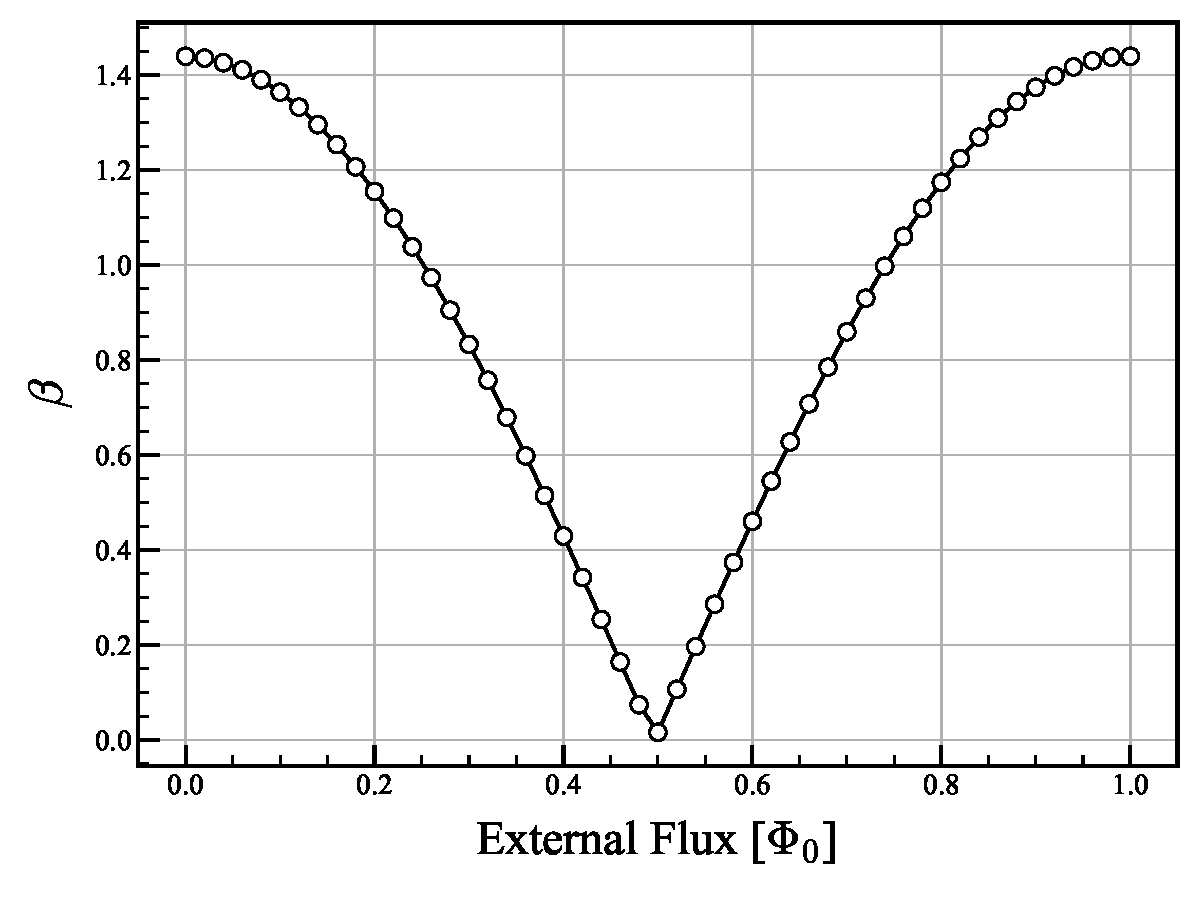
\includegraphics[width=9cm]{dc-squid.pdf}
            \caption{エネルギースペクトル}
        \end{figure}
        ではこのdc-SQUIDによってどのようジョセフソンインダクタンスが変化するのかを示す。
    \subsection{カイネティックインダクタンス}
        カイネティックインダクタンスは超伝導インダクタンスとも呼ばれる。超伝導細線を扱うとこのインダクタンスの影響が大きくなる。超伝導体中の準粒子移動により誘導されるインダクタンスである。このカイネティックインダクタンスは物質固有の値であり、非常に局所的な領域で大きなインダクタンスを得られるため、この特性を利用した量子ビットなども存在する。今回限られた設計内でおおきなインダクタンスを得るためにこのカイネティックインダクタンスを導入した。次節導入するミアンダインダクタンスは1μで加工されており、カイネティックインダクタンスの影響が大きく現れるとよそうされる。
    \subsection{ミアンダインダクタンス}
        ミアンダとは蛇行したという意味である。図の通り単純な直線ラインではなく折り返し構造を繰り返すことで、実質的な長さ、ライン間の相互インダクタンスにより総合的な自己インダクタンスが大きくなる。このミアンダインダクタンスを導入する上で論文の解析を利用した。計算方法を補足に記したので参照されたい。計算結果のみを示すと下図の構造に与えられた数値を入力することで得たいインダクタンスを求めることが可能である。次章でも言及するがこのミアンダインダクタンスの数値を考える上でもう一つ電磁界シミュレーションによる方法もとったのでここで紹介する。
        電磁界シミュレーションにはnational instruments社のマイクロウェーブオフィスを利用している。CADファイルで設定されたオブジェクトに材質特性を付与し電磁波の入出ポートを設定することで反射特性等を計算することが可能である。
        ここでシミュレーションする構造物は下図のようなミアンダインダクタンスのない単体の共振器とミアンダインダクタンスを導入した単体の共振器である。この2つのこの構造物全体のアドミッタンスを低周波数領域で計算することで構造物全体の伝導伝導性を計算することができる。アドミッタンス値からおおよその構造物のインダクタンスを計算することができるが2つの構造物の差分はおおよそミアンダインダクタンスの可否に依存する。そこでミアンダの数に対してインダクタンスがどれだけ増加するかプロットしたものが図である。この図からはミアンダの数に依存して線形にインダクタンスが増加していることがわかる。ここで上述した解析計算とどれだけの差があるかも同時にい示す。

        プロットの結果では0-100の範囲内で両者の乖離はおよそOOであった。さほど乖離はないといえるが参考値程度にとどめておく。今回のサンプル作成ではN=38をミアンダインダクタンスとして採用した。

\section{物理モデル}
ここまで紹介した超伝導素子を用いて本研究にて開発した結合素子の物理モデルを解説する。
\begin{figure}[H]
    \centering
    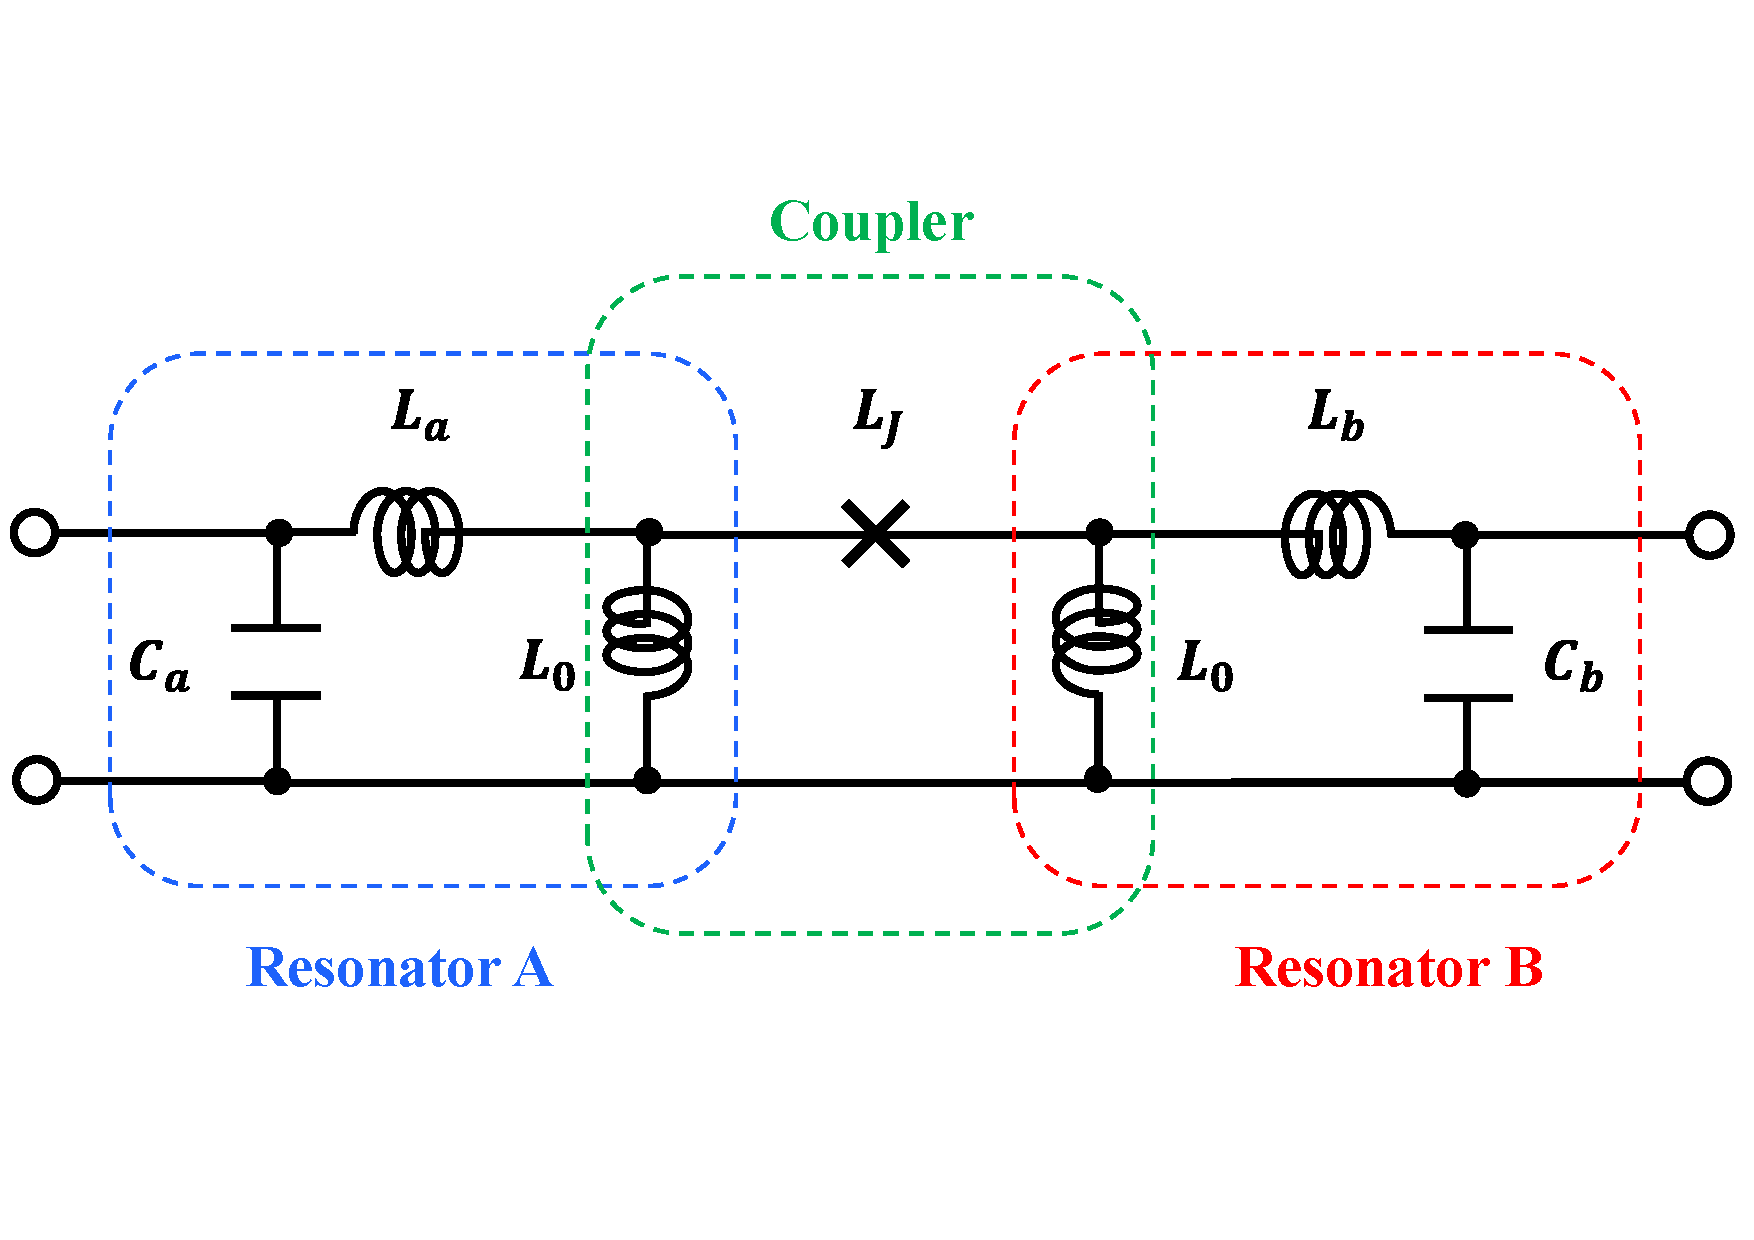
\includegraphics[width=14cm]{theory_circuit1_1.pdf}
    \caption{circuit1}
\end{figure}
図は本研究においてベーシックとなる回路である。2つのLC共振回路をジョセフソン接合を介して結合している。ジョセフソン接合は共振器間にループを為すように配置されている。この結合共振回路のハミルトニアンを2通りの異なるアプローチで導出する。
1つはrf-SQUIDを独立な素子として扱い、従来の伝送線路-超伝導ループ間の相互作用から類推してハミルトニアンを導出する方法。
もう1つの方法は結合回路を2端子対回路として回路の等価変換を行い、rf-SQUIDを変圧器的に扱いハミルトニアンを導出する方法である。2端子対回路のマトリックス表示に関する基本的な計算方法、また本結合回路を解析する際に用いた基本的な考え方(変圧器の磁気的結合回路、$T-\Pi$変換($Y-\Delta$変換)等)は補足に記載したため参考されたい。
\subsection{回路の等価変換に依る方法}
さて、本研究に於ける結合回路素子においても上記の古典的計算は応用ができる\cite*{Tian_2008}。本研究において、2つの共振器とrf-SQUIDがガルバニックに結合した系の結合部を以下のように書き表す。
\begin{figure}[H]
    \begin{minipage}[t]{0.5\columnwidth}
        \centering
        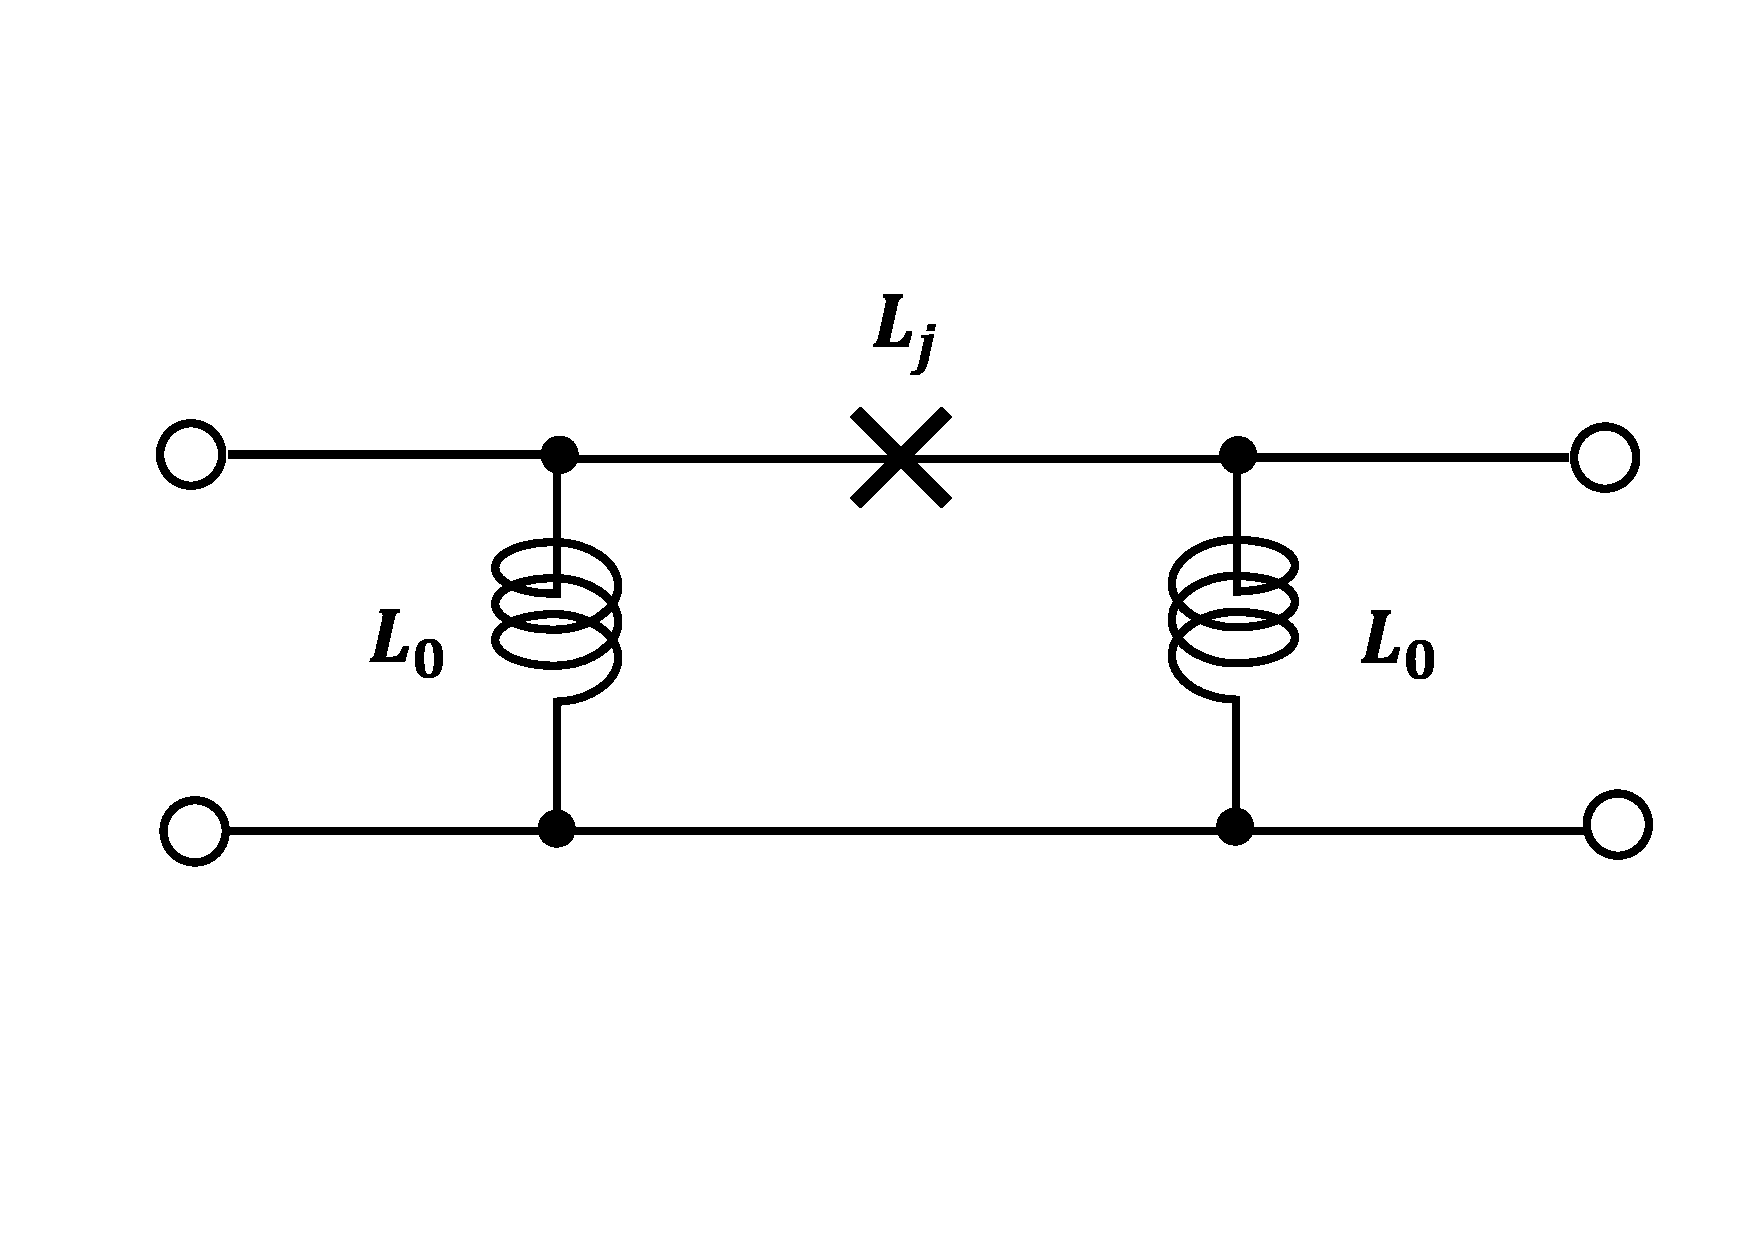
\includegraphics[clip, width=1.0\columnwidth]{circuit1.pdf}
        \caption{rf-SQUIDの回路表現}
    \end{minipage}%
    \begin{minipage}[t]{0.5\columnwidth}
        \centering
        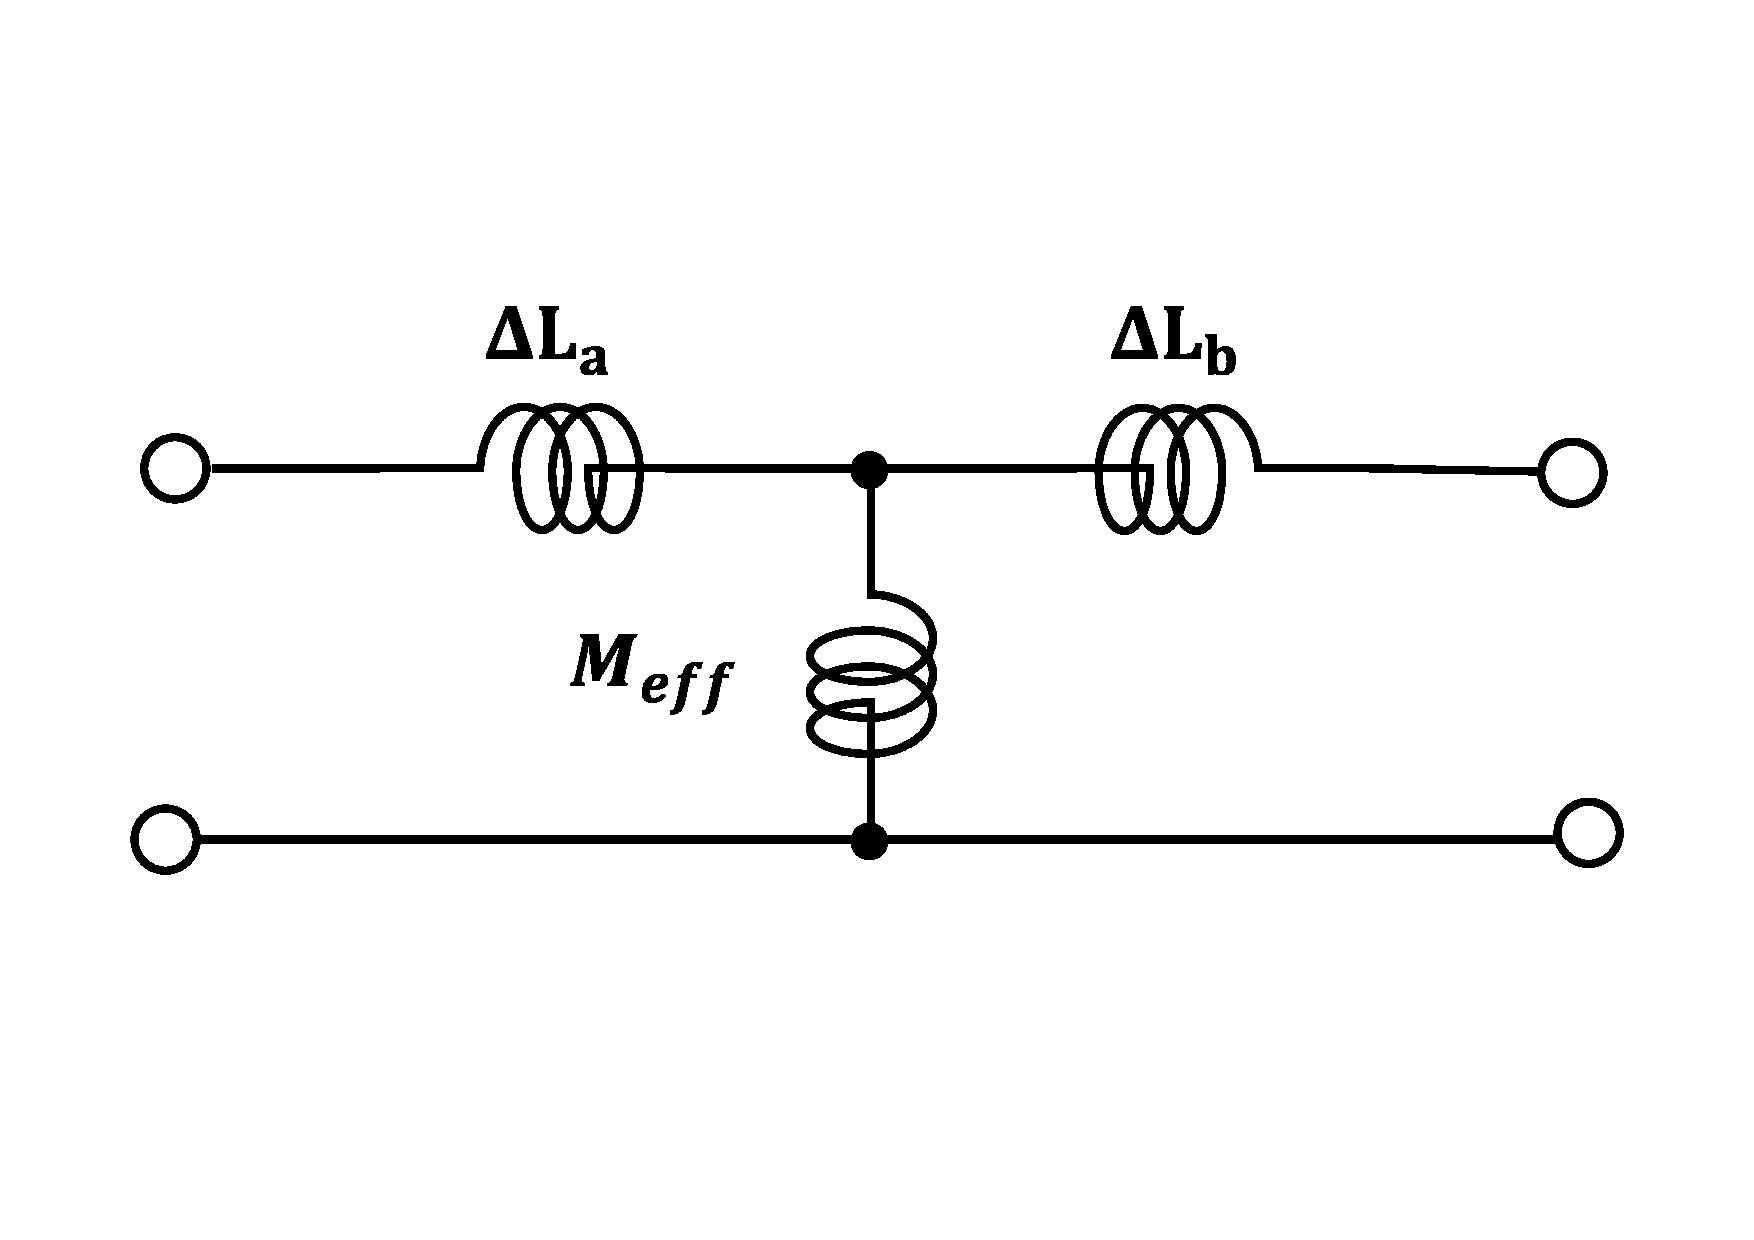
\includegraphics[clip, width=1.0\columnwidth]{circuit2.pdf}
        \caption{T型回路}
    \end{minipage}
\end{figure}
ここで簡便のためにジョセフソン接合はインダクタンス$L_J = L_{J0}/\cos (\phi)$として扱う。つまりジョセフソン接合は十分に小さいものとして扱い、接合の自己キャパシタンス$C_j$は小さいものとして無視する。このようにするとrf-SQUIDが共振器にガルバニックに相互インダクタンス$L_0$で結合していた場合、これは$\Pi$型の2端子対回路であることがわかる。今ジョセフソンインダクタンスを接合の位相差$\phi$に依存する非線形なインダクタンスとして扱うと$\Pi-T$変換にしたがって図中の実行相互インダクタンス$M_{eff}$は

\begin{eqnarray}
    M_{eff}(\phi) & = \frac{L_0^2}{Ls+Lj(\phi)}\\
    & =\frac{L_0^2}{L_{rf}(\phi)}
\end{eqnarray}
となる。ここで$L_S$はrf-SQUIDの自己インダクタンスであり、$L_S = 2 L_0$である。
また、
\begin{eqnarray}
    L_{rf}(\phi)  &=& Ls+\frac{L_{J0}}{\cos (\phi)}\\ \\
    &=& \frac{L_S \cos (\phi)+L_{J0}}{\cos (\phi)}\\ \\
    &=& \frac{\frac{L_S^2}{L_{J0}} \cos (\phi)+L_S}{\frac{L_S}{L_{J0}}\cos (\phi)}\\ \\
    &=& \frac{L_S(\beta \cos (\phi)+1)}{\beta \cos (\phi)}
\end{eqnarray}
この時両共振器間には実行的にインダクタンス$M_{eff}$を介してエネルギーの交換を行う。
相互作用ハミルトニアンは
\begin{equation}
    H_{\mathrm{int}}(\phi)=-M_{\mathrm{eff}}(\phi) \sqrt{\frac{\hbar \omega_{a}}{2 L_{a}} \frac{\hbar \omega_{b}}{2 L_{b}}}\left(\hat{a}+\hat{a}^{\dagger}\right)\left(\hat{b}+\hat{b}^{\dagger}\right)
\end{equation}
$L_{a,b}$は各共振器のインダクタンス、$\omega_{a,b}$は共振周波数$a\dagger,a,b,b\dagger$は各共振器の生成消滅演算子である。

\begin{figure}[H]
    \begin{minipage}[t]{0.5\columnwidth}
        \centering
        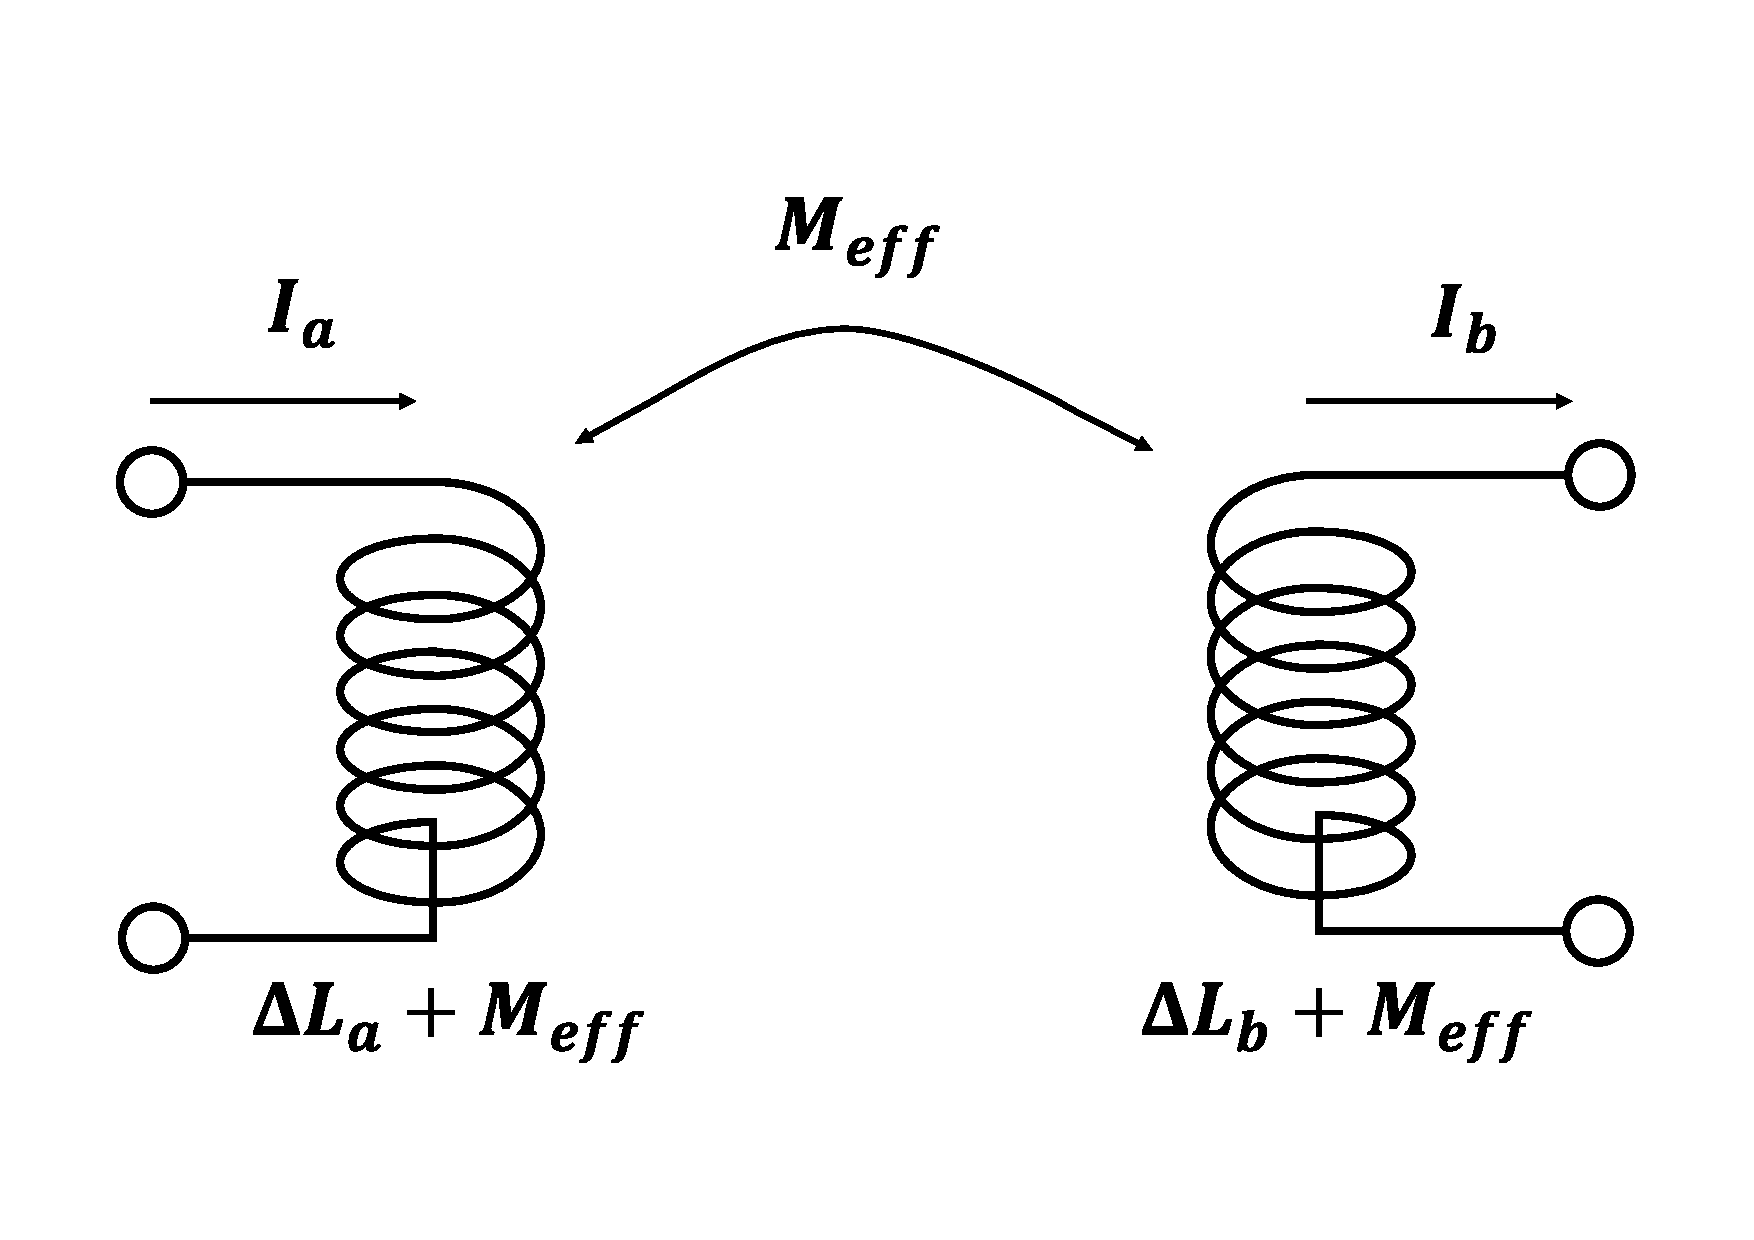
\includegraphics[clip, width=1.0\columnwidth]{circuit3.pdf}
        \caption{分離}
    \end{minipage}%
    \begin{minipage}[t]{0.5\columnwidth}
        \centering
        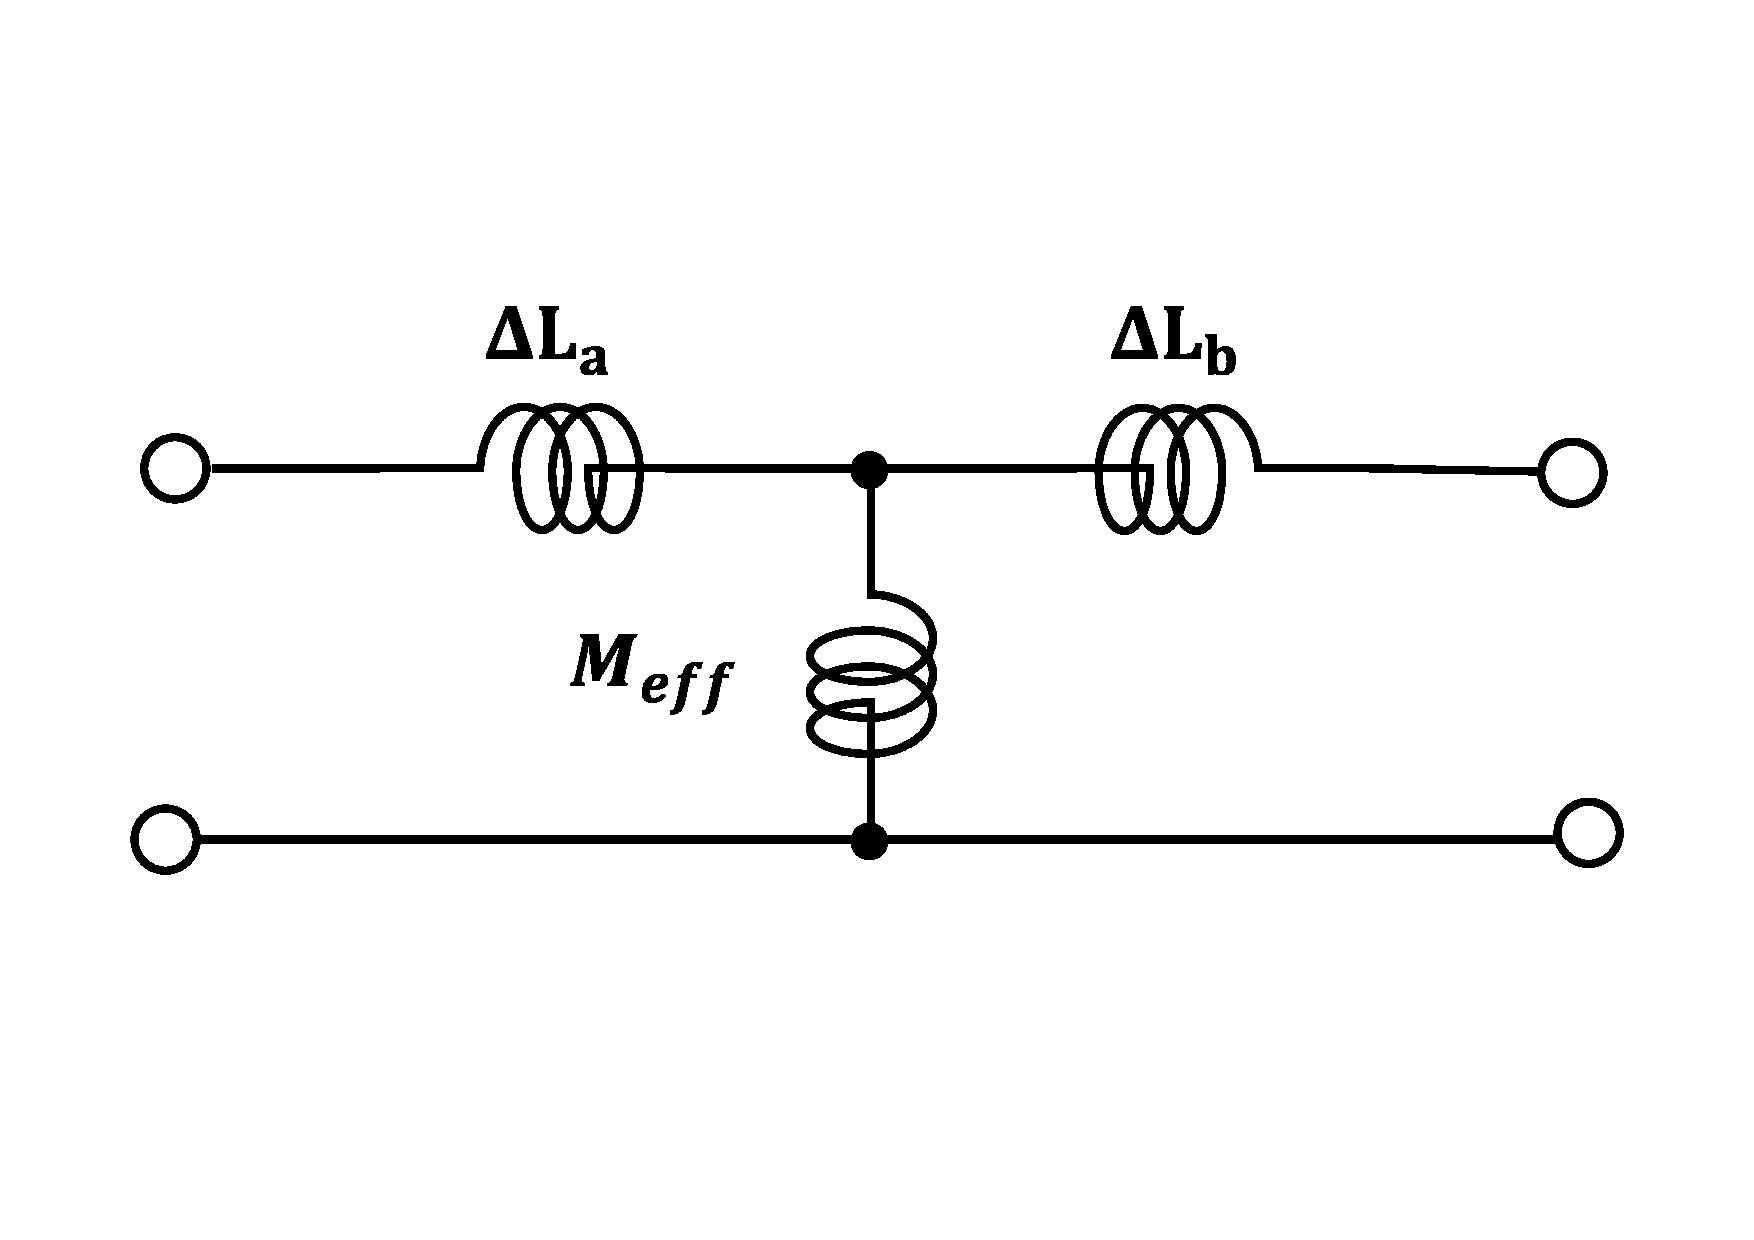
\includegraphics[clip, width=1.0\columnwidth]{circuit2.pdf}
        \caption{T型回路}
    \end{minipage}
\end{figure}
この時$\Delta L_{a,b}$は

\begin{equation}
    \Delta L_{a,b} = \frac{L_0L_J}{2L_0+L_J} = \frac{L_0L_J}{L_S+L_J} = \frac{L_0L_J}{L_{rf}}
\end{equation}

である。T型回路を相互インダクタンス$M_{eff}$で結合している2つの共振素子に再び分離すると共振素子は元のインダクタンス$L_{a,b}$から$\Delta L_a + M_{eff}$だけシフトする。シフトする周波数は

\begin{eqnarray}
    \Delta L_{a,b} + M{eff} & = &  \frac{L_0L_J}{2L_0+L_J} + \frac{L_0^2}{2L_0+L_J}\\ \\
    & = & \frac{L_0 L_J + L_0^2}{L_S + L_J}\\ \\
    & = & \frac{L_0 L_{J0}/\cos (\phi) + L_0^2}{L_S + L_{J0}/\cos (\phi)}\\ \\
    & = & \frac{L_0 L_{J0} + L_0^2 \cos (\phi)}{L_S \cos (\phi) + L_{J0}}\\ \\
    & = & \frac{L_0 + L_0^2/L_{J0} \cos (\phi)}{L_S/L_{J0} \cos (\phi) + 1}\\ \\
    & = & \frac{L_0^2}{L_S}\frac{2 + \beta \cos (\phi)}{1+\beta \cos (\phi)}
\end{eqnarray}

ここで

\begin{equation}
    L_S = 2L_{J0}
\end{equation}

を用いた。元の共振素子は結合部以外で$L_{a,b}$のインダクタンスを保有していたため、共振周波数は

\begin{equation}
    \omega_a = \frac{1}{\sqrt{L_aC_a}}
\end{equation}

である。結合により生じたシフト分を考慮すると、それぞれの共振周波数は

\begin{eqnarray}
    \tilde{\omega_{a,b}} &=&  \frac{1}{\sqrt{(L_a+\frac{L_0^2}{L_S}\frac{2 + \beta \cos (\phi)}{1+\beta \cos (\phi)})C_a}}\\ \\
    & = &  \frac{1}{\sqrt{L_{a,b}C_{a,b}}} \frac{1}{\sqrt{1+\frac{L_0^2}{L_{a,b}L_S}\frac{2 + \beta \cos (\phi)}{1+\beta \cos (\phi)}}}\\ \\
    & = &  \omega_{a,b} \biggl(1+\frac{L_0^2}{L_{a,b}L_S}\frac{2 + \beta \cos (\phi)}{1+\beta\ cos(\phi)}\biggr)^{-\frac{1}{2}}\\ \\
    & = &  \omega_{a,b} \biggl(1-\frac{L_0^2}{2L_{a,b}L_S}\frac{2 + \beta \cos (\phi)}{1+\beta\ cos(\phi)}\biggr)
\end{eqnarray}

各共振器を流れる電流は

\begin{equation}
    I_{a,b} = \sqrt{\frac{f_{a,b}}{2 L_{a,b}}}
\end{equation}

であるから、結合強度$g(\phi)$を
\begin{equation}
    g(\phi) = (M_{eff}+M{ab})I_a I_b
\end{equation}
とすることで回路のハミルトニアンを
\begin{equation}
    \hat{\mathcal{H}} = \hbar \hat{\omega}_{a} \hat{a}^{\dagger} \hat{a}+\hbar \hat{\omega}_{b} \hat{b}^{\dagger} \hat{b}+\hbar g(\Phi)\left(\hat{a}^{\dagger}\hat{b}+\hat{a} \vec{b}^{+}\right)
\end{equation}
のように書き表すことができる。ここで$M_{ab}$は共振器間の1次結合であり、これは共振器同士の距離に強く依存する。そのため、結合の正成分を大きくするためには共振器感の物理的距離を考慮することが肝要である。

以上のハミルトニアンから回路の遷移エネルギーを計算すると


\subsection{rf-SQUIDの性質から求める方法}
次にrf-SQUIDの性質より求める方法である。rf-SQUIDは既に説明したようにジョセフソン接合1つを含んだ超伝導ループである。超伝導ループの自己インダクタンスを$L_S$、ループを流れる臨界電流を$I_C$とする。ループを外部磁束が貫くとループの自己インダクタンスにより外部磁束を打ち消す方向に遮蔽電流が流れる。

\begin{equation}
    I_{S}(\Phi)=I_{c} \sin \left(2 \pi \Phi / \Phi_{0}\right)
\end{equation}

ここでループを貫く磁束は外部磁束とループの自己インダクタンスによる遮蔽磁場の和である。

\begin{equation}
    \Phi=\Phi_{\text {ext }}-L_{S} I_{S}(\Phi)
\end{equation}

以上の関係式よりrf-SQUIDが持つ実効的なインダクタンスを求めることができる。実効インダクタンスを$L_{rf}(\Phi)$とすると外部磁束の変化に於ける遮蔽電流の変化量から

\begin{equation}
    \frac{1}{L_{rf}(\Phi)}=\frac{\partial I_{S}}{\partial \Phi_{\mathrm{ext}}}=\frac{\partial I_{S}}{\partial \Phi} \frac{\partial \Phi}{\partial \Phi_{\mathrm{ext}}}
\end{equation}

となる。ここで

\begin{equation}
    \frac{\partial I_S}{\partial \Phi} = \frac{2\pi I_C}{\Phi_0} cos (2 \pi \Phi / \Phi_0)
\end{equation}

\begin{equation}
    \frac{\partial \Phi}{\partial \Phi_{ext}} = 1 - L_S\frac{\partial I_S}{\partial \Phi_{ext}}
\end{equation}

\begin{equation}
    \beta = \frac{2\pi L_S I_C}{\Phi_0}
\end{equation}

であることを用いると

\begin{equation*}
    \frac{\partial I_S}{\partial \Phi_{ext}} = \frac{\beta}{L_S}\cos (2\pi \Phi/\Phi_0)-\beta \cos (2\pi \Phi / \Phi_0) \frac{\partial I_S}{\partial \Phi_{ext}}
\end{equation*}

\begin{equation*}
    \biggl(1+\beta \cos (2\pi \Phi / \Phi_0)\biggr)\frac{\partial I_S}{\partial \Phi_{ext}} = \frac{\beta}{L_S}\cos (2\pi \Phi / \Phi_0)
\end{equation*}

\begin{equation*}
    \frac{1}{L_{rf}(\Phi)}=\frac{\partial I_S}{\partial \Phi_{ext}} = \frac{1}{L_{S}} \frac{\beta \cos \left(2 \pi \Phi/\phi_{0}\right)}{1+\beta \cos \left(2 \pi \Phi/\phi_{0}\right)}
\end{equation*}

が導かれる。回路の等価変換に依る方法と同じ帰結が得られたことがわかる。\\
この時、共振器に流れる電流$I_{a,b}$はrfSQUIDに流入し、磁気的な結合をもたらす。電流$I_{a,b}$により生じる磁束を$\Phi_{a,b}$とすると相互作用ハミルトニアンは

\begin{equation}
    H_{\text {ind }}=\frac{\left(\Phi_{a}-\Phi_{b}\right)^{2}}{2 L_{rf}(\Phi)}=\frac{\Phi_{a}^{2}+\Phi_{b}^{2}-2 \Phi_{b} \Phi_{b}}{2 L_{rf}(\Phi)}
\end{equation}

となる。相互作用ハミルトニアンのうち、$\Phi_{a,b}^2$の項は共振周波数のシフトをもたらす。シフトされた共振周波数は

\begin{equation}
    \tilde{\omega}_{a,b}=\omega_{a,b} \sqrt{1-2 \frac{L_{0}^{2}}{L_{a,b} L_{rf}(\Phi)}} \approx \omega_{a,b}\left(1-\frac{L_{0}^{2}}{L_{a,b} L_{rf}(\Phi)}\right)
\end{equation}

であり、各々の共振器に流れる電流によりrf-SQUIDを介して結合

\begin{equation}
    g(\Phi)=-\underbrace{\sqrt{\frac{\omega_{a}}{L_{a}}}}_{I_{a}} \underbrace{\sqrt{\frac{\omega_{b}}{L_{b}}}}_{I_{b}} \underbrace{\frac{L_{0}^{2}}{L_{r f}(\Phi)}}_{M_{eff}}
\end{equation}

が生じている。共振器間の磁気的結合に依る1次結合を考慮すると結合強度の総和は

\begin{equation}
    g_{eff}(\Phi)=g(\Phi)+g_{ab}
\end{equation}

となり、系のハミルトニアンは
\begin{subequations}
    {\jot=10pt
\begin{eqnarray}
    \hat{\mathcal{H}}&=&\hbar\biggl(\hat{a}^{\dagger }\ \hat{b}^{\dagger }\biggr)\biggl(\begin{array}{cc}
    \tilde{\omega}_{a} & g_{eff}(\Phi ) \\
    g_{eff}(\Phi ) & \tilde{\omega}_{b}
    \end{array}\biggr)\biggl(\begin{array}{l}
    \hat{a} \\
    \hat{b}
    \end{array}\biggr)\\
    &=& \hbar \tilde{\omega}_{a} \hat{a}^{\dagger} \hat{a}+\hbar \tilde{\omega}_{b} \hat{b}^{\dagger} \hat{b}+\hbar g_{eff}(\Phi)\biggl(\hat{a}^{\dagger}\hat{b}+ \hat{b}^{\dagger}\hat{a}\biggr)
\end{eqnarray}
}
\end{subequations}
となる。\\
上式から、rf-SQUIDによりエネルギーシフトした共振器同士は結合項$g_{eff}(\Phi)$で結合している。ただし、実際の測定環境では各々の共振器の共振エネルギーではなく、2つの共振器が結合したモードとして観測が為される。そこで上式をさらに式変形する。
結合したモードの基底を

\begin{equation}
    \hat{c}_{\pm}=\frac{\hat{a} \pm \hat{b}}{\sqrt{2}} ,\quad \hat{c}_{\pm}^{\dagger}=\frac{\hat{a}^{\dagger} \pm \hat{b}^{\dagger}}{\sqrt{2}}
\end{equation}

のように書き表す。$\hat{c}_{\pm}^{\dagger},\hat{c}_{\pm}$は結合モードの生成消滅演算子である。詳細な計算は冗長になるため、補足に預けることとする。
この新たな基底によりハミルトニアンの変換を行うと
\begin{subequations}
    {\jot=10pt
\begin{eqnarray}
    \hat{H}&=&\hbar\Omega_{+} \hat{c}_{+}^{\dagger} \hat{c}_{+}+\hbar\Omega_{-} \hat{c}_{-}^{\dagger} \hat{c}_{-} +\hbar \Delta \biggl(\hat{c}_{+}^{\dagger}\hat{c}_{-}-\hat{c}_{-}^{\dagger} \hat{c}_{+}\biggr)\\
    &=& \hbar\biggl(\begin{array}{cc}
        \hat{c}_{+}^{\dagger} & \hat{c}_{-}^{\dagger}
        \end{array}\biggr)\biggl(\begin{array}{cc}
        \Omega_{+} & \Delta \\
        \Delta & \Omega_{-}
        \end{array}\biggr)\biggl(\begin{array}{l}
        \hat{c}_{+} \\
        \hat{c}_{-}
        \end{array}\biggr)
\end{eqnarray}
}
\end{subequations}
という式が得られる。ここで
ここで第1項と第2項について
\begin{equation}
    \Omega_{+}=\frac{\tilde{\omega}_{a}+\tilde{\omega}_{b}}{2} + g_{eff}(\Phi)
\end{equation}
\begin{equation}
    \Omega_{-}=\frac{\tilde{\omega}_{a}+\tilde{\omega}_{b}}{2} - g_{eff}(\Phi)
\end{equation}
第3項について
\begin{equation}
    \Delta = \frac{\tilde{\omega}_{a}-\tilde{\omega}_{b}}{2}
\end{equation}
であることに注意する。すなわち結合系において共振器A,Bの結合強度は新たな基底の固有モードの差分の半分
\begin{equation}
    g_{eff}(\Phi)=\frac{\Omega_{+}-\Omega_{-}}{2} 
\end{equation}
に相当することがわかる。
このハミルトニアンの遷移周波数をプロットを以下に示す。
\begin{figure}[H]
    \begin{minipage}[t]{0.5\columnwidth}
        \centering
        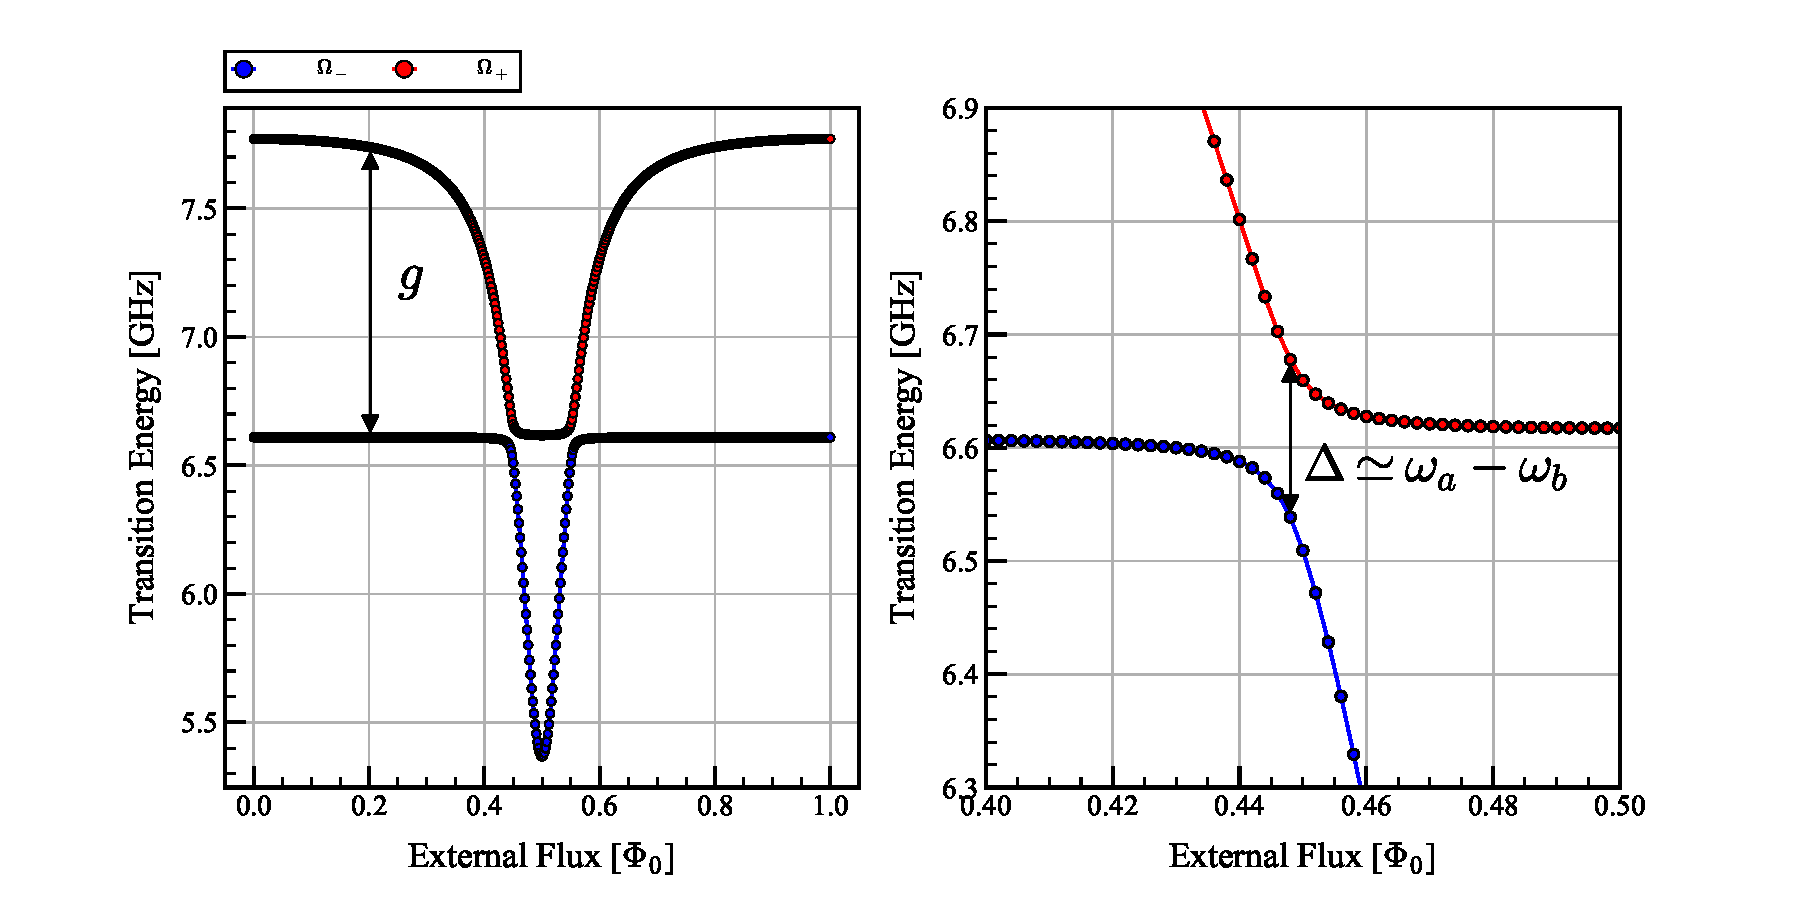
\includegraphics[clip, width=1.0\columnwidth]{standard_eigen.pdf}
        \caption{遷移周波数}
    \end{minipage}%
    \begin{minipage}[t]{0.5\columnwidth}
        \centering
        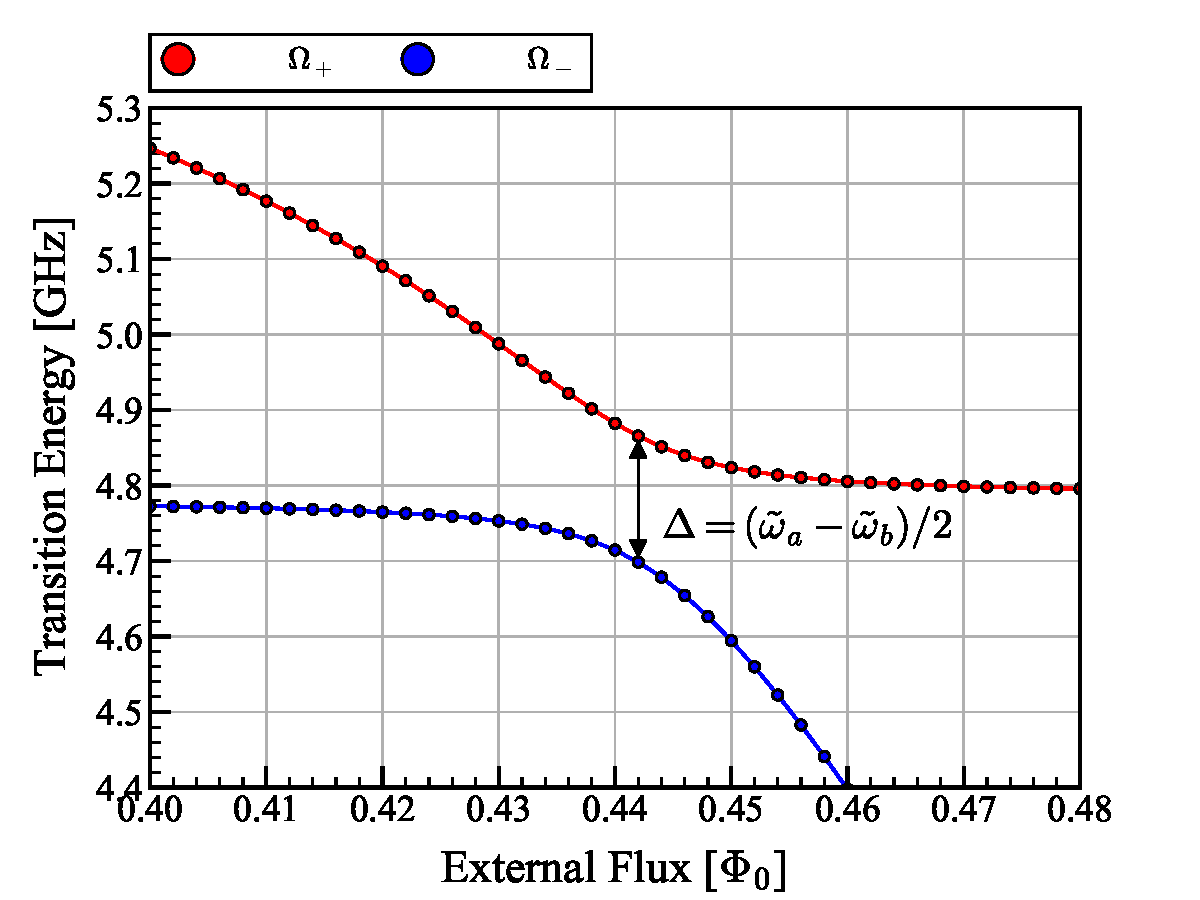
\includegraphics[clip, width=1.0\columnwidth]{standard_eigen_zoom.pdf}
        \caption{結合強度ゼロ付近の拡大図}
    \end{minipage}
\end{figure}
測定についても以上の性質を利用する。すなわち結合モードの遷移周波数を上記ハミルトニアンでフィットし結合定数を見積もる。
つまり、このパラメータに於ける結合強度をプロットすると
\begin{figure}[H]
    \begin{minipage}[t]{0.5\columnwidth}
        \centering
        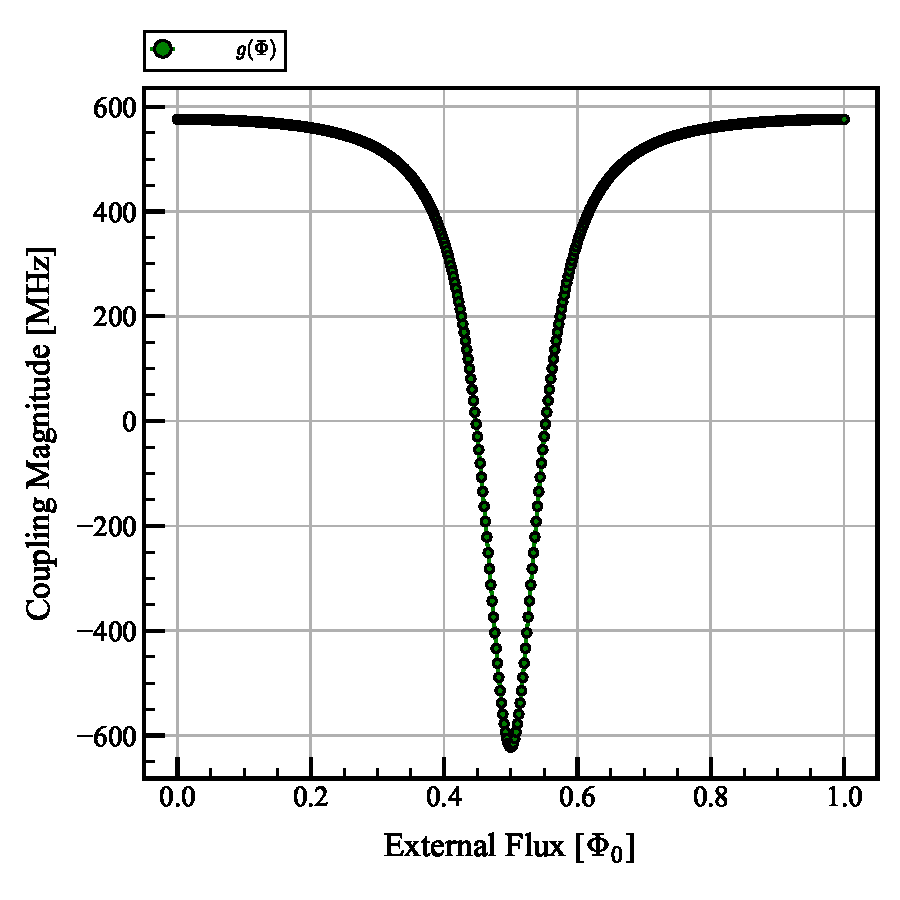
\includegraphics[clip, width=1.0\columnwidth]{standard_coupling.pdf}
        \caption{結合強度}
    \end{minipage}%
    \begin{minipage}[t]{0.5\columnwidth}
        \centering
        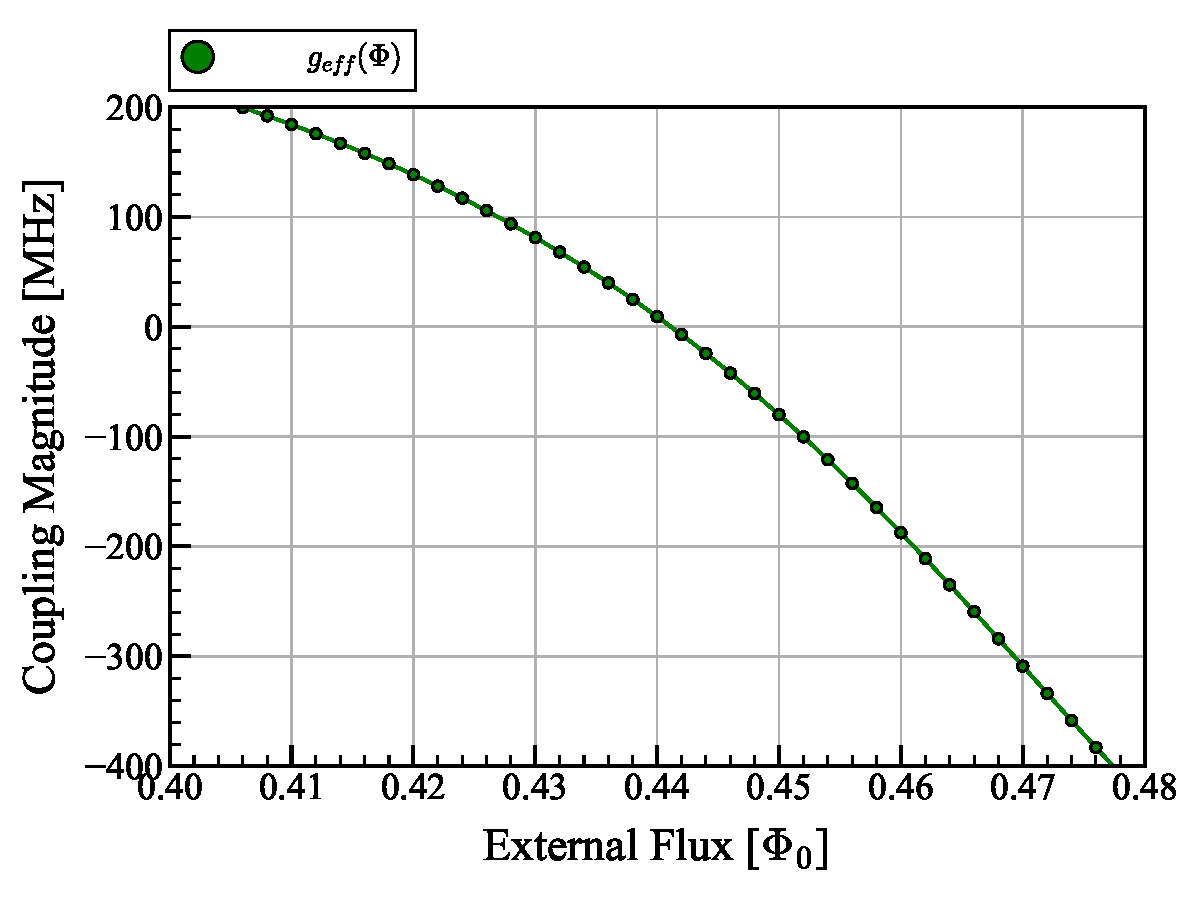
\includegraphics[clip, width=1.0\columnwidth]{standard_coupling_zoom.pdf}
        \caption{結合強度ゼロ付近の拡大図}
    \end{minipage}
\end{figure}
のようになる。
上記の結合モードの遷移周波数$\Omega_{+},\Omega_{-}$のプロットにrf-SQUIDによって変調された共振器A,Bの遷移周波数$\tilde{\omega}_a,\tilde{\omega}_b$をプロットすると
\begin{figure}[H]
    \begin{minipage}[t]{0.5\columnwidth}
        \centering
        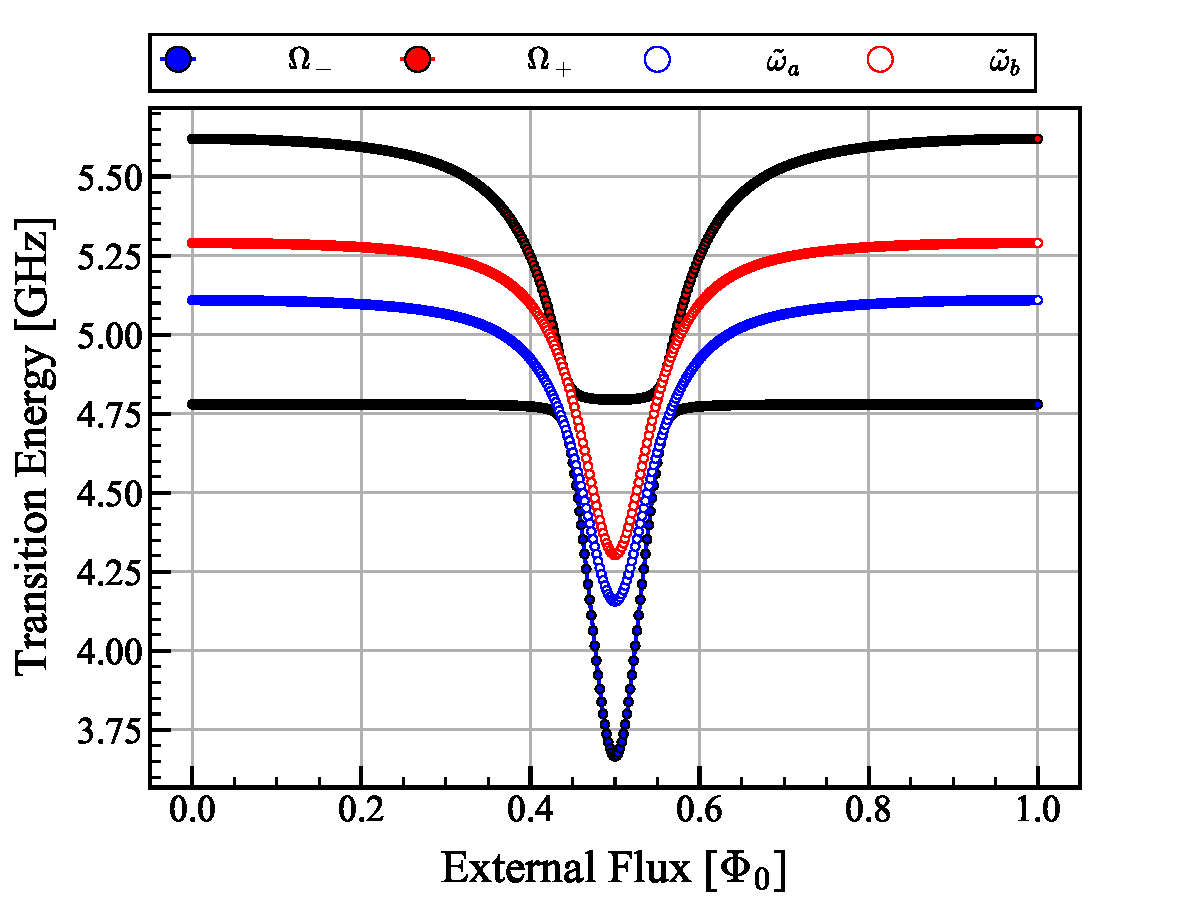
\includegraphics[clip, width=1.0\columnwidth]{standard_eigen_with.pdf}
        \caption{遷移周波数}
    \end{minipage}%
    \begin{minipage}[t]{0.5\columnwidth}
        \centering
        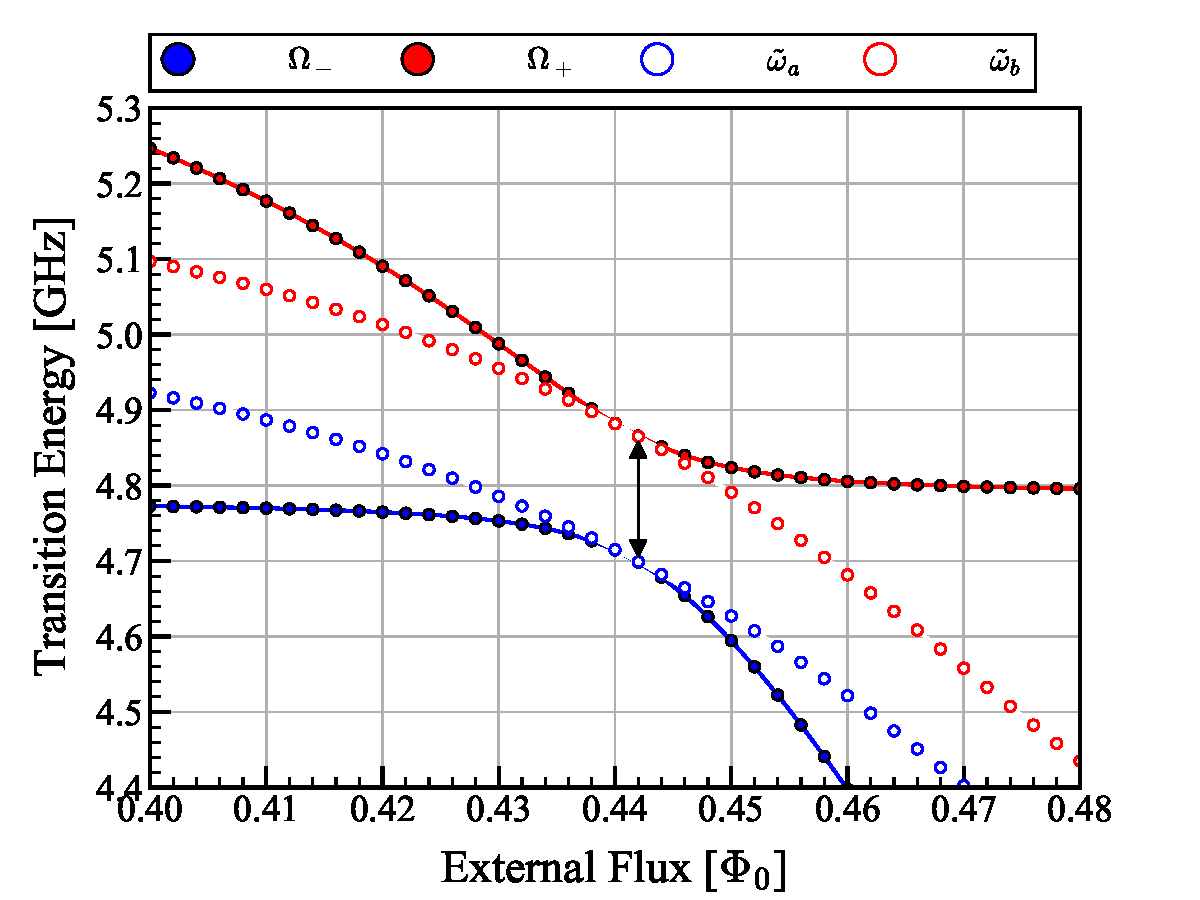
\includegraphics[clip, width=1.0\columnwidth]{standard_eigen_with_zoom.pdf}
        \caption{結合強度ゼロ付近の拡大図}
    \end{minipage}
\end{figure}
以上のプロットより、結合強度がゼロとなる点において結合モードの遷移周波数$\Omega_{+},\Omega_{-}$とrf-SQUIDによって変調された共振器A,Bの遷移周波数$\tilde{\omega}_a,\tilde{\omega}_b$が一致することがわかる。すなわち、この点において共振器A,Bは完全に独立た状態であるとみなすことができる。

このことは共振器A,Bの状態を外部磁束に対してトレースすることでも理解できる。
すなわち共振器A,Bの混合比を次のように定義する
\begin{equation}
    Mix\ Ratio\ \Omega_{-} = A:B  = \biggl|\left\langle \tilde{\psi}_a|\Psi_{-}\right\rangle \biggr|^2: \  \biggl|\left\langle \tilde{\psi}_b|\Psi_{-}\right\rangle \biggr|^2 
\end{equation}
\begin{equation}
    Mix\ Ratio\ \Omega_{+} = A:B  = \biggl|\left\langle \tilde{\psi}_a|\Psi_{+}\right\rangle \biggr|^2: \  \biggl|\left\langle \tilde{\psi}_b|\Psi_{+}\right\rangle \biggr|^2 
\end{equation}

ここで$\tilde{\psi}_{a,b}$,$\Psi_{+,-}$はそれぞれ共振モード$\tilde{\omega}_a,\tilde{\omega}_b$、$\Omega_{+},\Omega_{-}$の波動関数である。すなわち混合比は結合モードにおいて共振モード$\tilde{\omega}_a,\tilde{\omega}_b$がどれだけ存在するかの指標となっている。結合がゼロとなる点においては混合比はそれぞれ
\begin{equation}
    Mix\ Ratio\ \Omega_{-} = A:B  = 100: \  0
\end{equation}
\begin{equation}
    Mix\ Ratio\ \Omega_{+} = A:B  = 0: \  100
\end{equation}
となるはずである。\\
以下に結合モード$\Omega_{+},\Omega_{-}$中の混合比を示す。
\begin{figure}[H]
    \begin{minipage}[t]{0.5\columnwidth}
        \centering
        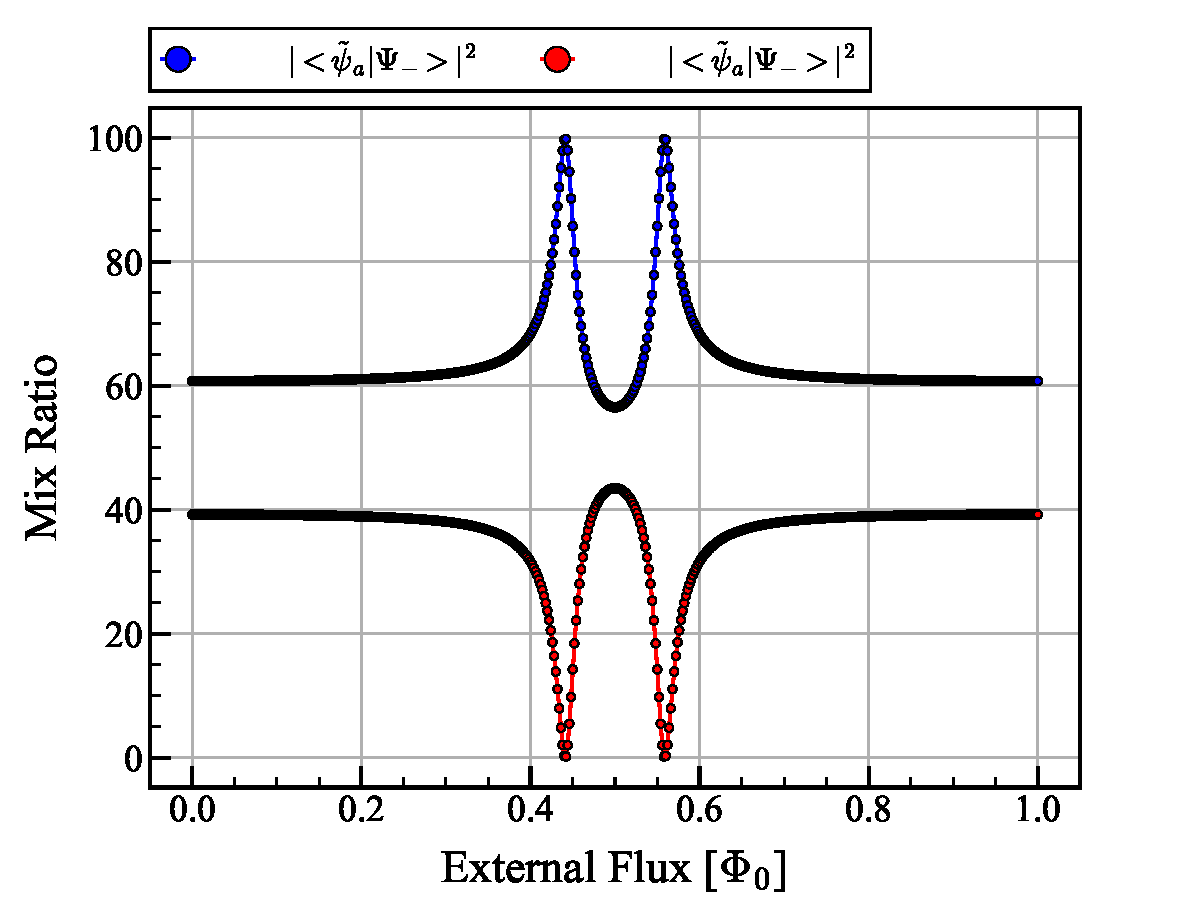
\includegraphics[clip, width=1.0\columnwidth]{MixRatio1.pdf}
        \caption{結合モード$\Omega_{-}$中の混合比}
    \end{minipage}%
    \begin{minipage}[t]{0.5\columnwidth}
        \centering
        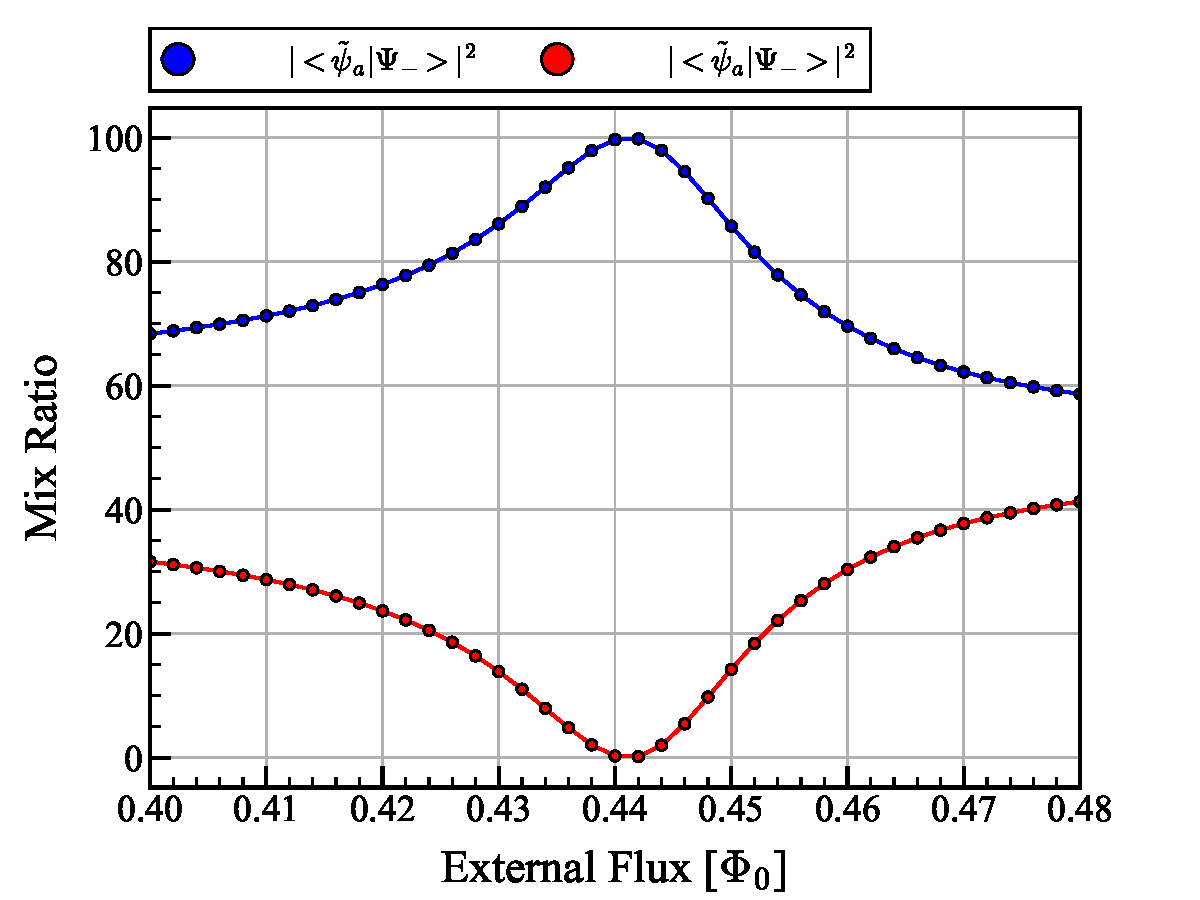
\includegraphics[clip, width=1.0\columnwidth]{MixRatio1_zoom.pdf}
        \caption{結合強度ゼロ付近の拡大図}
    \end{minipage}
\end{figure}
\begin{figure}[H]
    \begin{minipage}[t]{0.5\columnwidth}
        \centering
        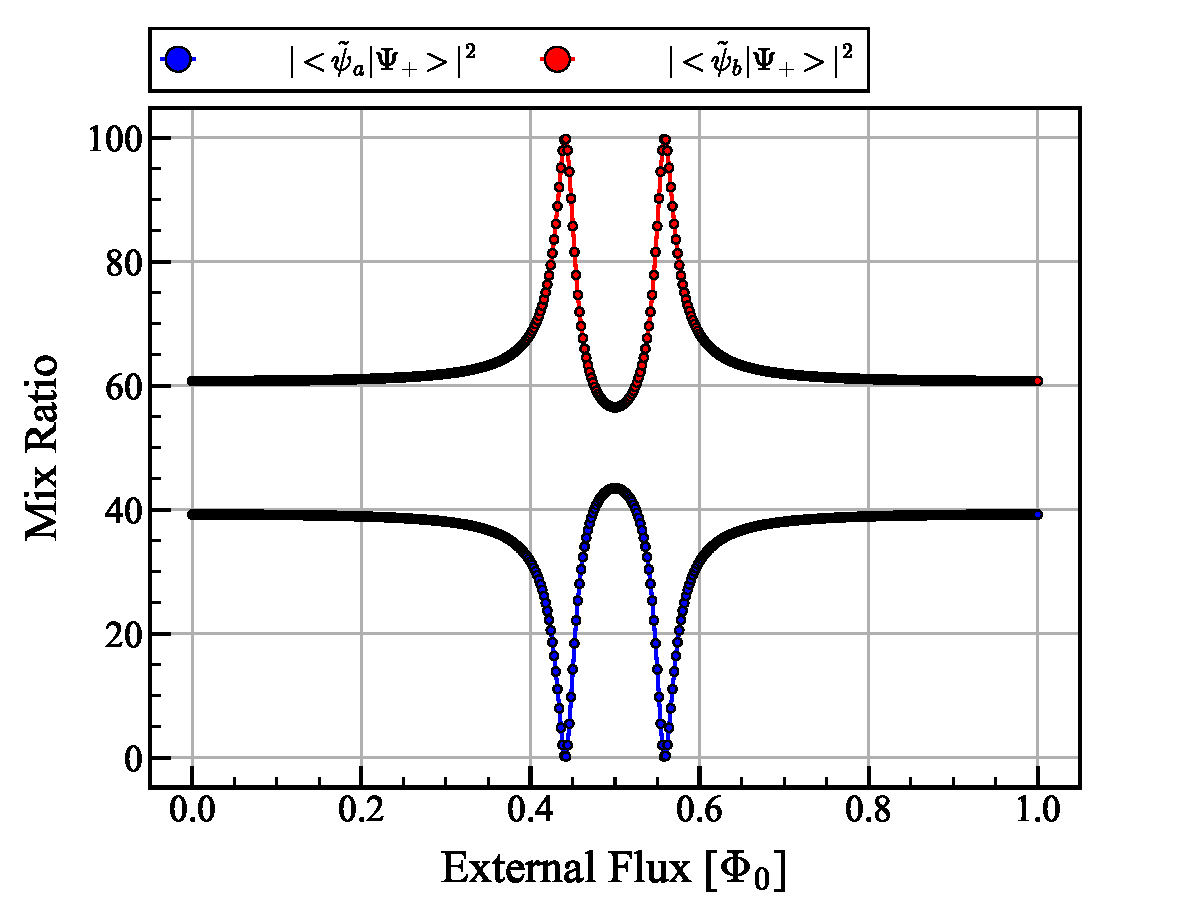
\includegraphics[clip, width=1.0\columnwidth]{MixRatio2.pdf}
        \caption{結合モード$\Omega_{+}$中の混合比}
    \end{minipage}%
    \begin{minipage}[t]{0.5\columnwidth}
        \centering
        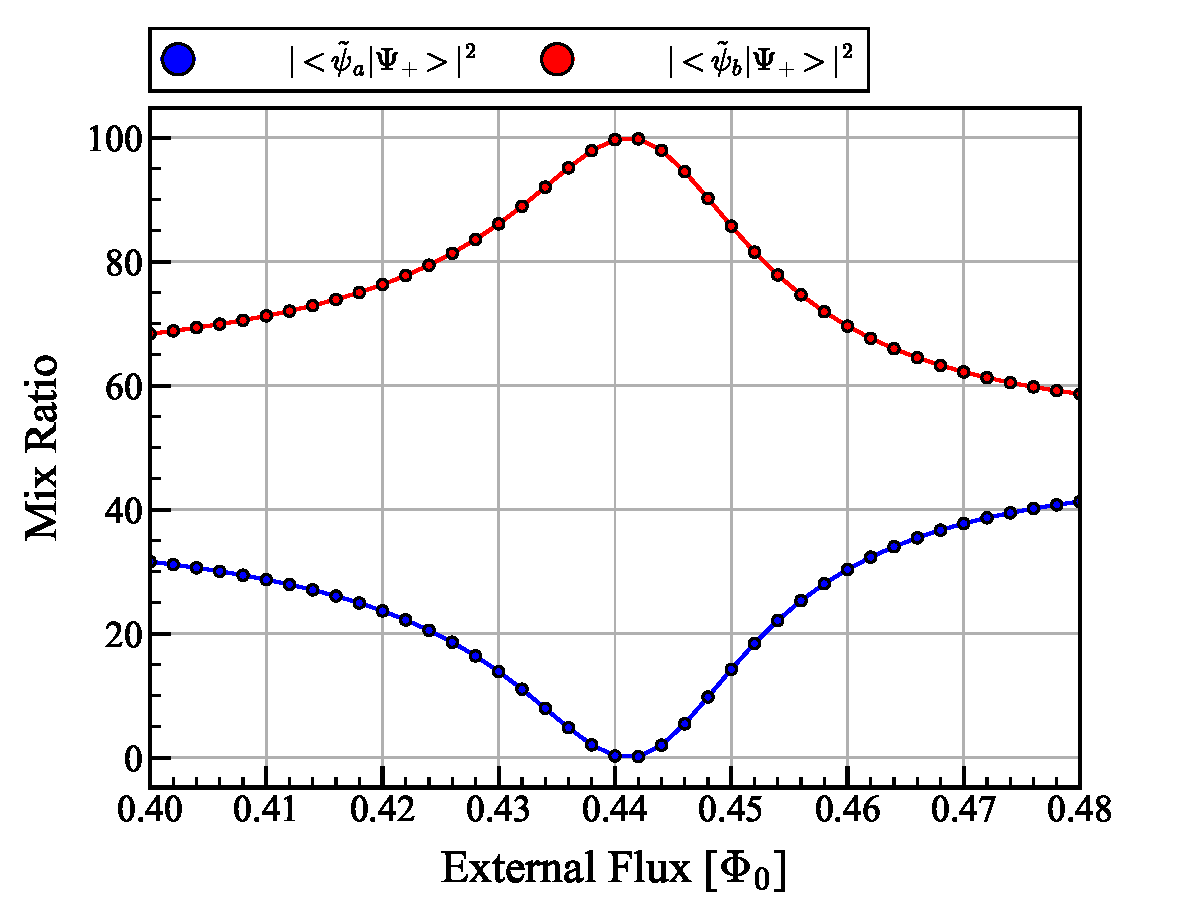
\includegraphics[clip, width=1.0\columnwidth]{MixRatio2_zoom.pdf}
        \caption{結合強度ゼロ付近の拡大図}
    \end{minipage}
\end{figure}